\documentclass[
	% -- opções da classe memoir --
	12pt,				% tamanho da fonte
	oneside,			% para impressão em verso e anverso. Oposto a oneside
	a4paper,			% tamanho do papel. 
	% -- opções da classe abntex2 --
	%chapter=TITLE,		% títulos de capítulos convertidos em letras maiúsculas
	%section=TITLE,		% títulos de seções convertidos em letras maiúsculas
	%subsection=TITLE,	% títulos de subseções convertidos em letras maiúsculas
	%subsubsection=TITLE,% títulos de subsubseções convertidos em letras maiúsculas
	% -- opções do pacote babel --
	english,			% idioma adicional para hifenização
	french,				% idioma adicional para hifenização
	spanish,			% idioma adicional para hifenização
	brazil,				% o último idioma é o principal do documento
	]{abntex2}


% ---
% PACOTES
% ---

% ---
% Pacotes fundamentais 
% ---
\usepackage{cmap}				% Mapear caracteres especiais no PDF
\usepackage{lmodern}			% Usa a fonte Latin Modern			
\usepackage[T1]{fontenc}		% Selecao de codigos de fonte.
\usepackage[utf8]{inputenc}		% Codificacao do documento (conversão automática dos acentos)
\usepackage{lastpage}			% Usado pela Ficha catalográfica
\usepackage{indentfirst}		% Indenta o primeiro parágrafo de cada seção.
\usepackage{color}				% Controle das cores
\usepackage{graphicx}			% Inclusão de gráficos
\usepackage[labelfont=bf,textfont=md]{caption}
\usepackage{amsmath}
% ---
		
% ---
% Pacotes adicionais, usados apenas no âmbito do Modelo Canônico do abnteX2
% ---
\usepackage{lipsum}				% para geração de dummy text
% ---

% ---
% Pacotes de citações
% ---
\usepackage[alf]{abntex2cite}	% Citações padrão ABNT

% --- 
% CONFIGURAÇÕES DE PACOTES
% --- 


% ---
% Informações de dados para CAPA e FOLHA DE ROSTO
% ---
\titulo{DESENVOLVIMENTO DE UMA FERRAMENTA GAMIFICADA PARA O ENSINO DE PROCESSAMENTO DIGITAL DE IMAGENS}
\autor{JONATA DANIEL BECKER}
\local{Novo Hamburgo}
\data{2018}
\orientador{Profa. Dra. Marta Rosecler Bez}
\instituicao{UNIVERSIDADE FEEVALE}
\tipotrabalho{Monografia}
% O preambulo deve conter o tipo do trabalho, o objetivo, 
% o nome da instituição e a área de concentração 
\preambulo{Trabalho de Conclusão de Curso apresentado como requisito parcial à obtenção do grau de Bacharel em Ciência da Computação pela Universidade Feevale}
% ---

% ---
% Configurações de aparência do PDF final

% alterando o aspecto da cor azul
\definecolor{blue}{RGB}{41,5,195}
\definecolor{black}{RGB}{0,0,0}

% informações do PDF
\makeatletter
\hypersetup{
     	%pagebackref=true,
		pdftitle={\@title}, 
		pdfauthor={\@author},
    	pdfsubject={\imprimirpreambulo},
	    pdfcreator={LaTeX with abnTeX2},
		pdfkeywords={abnt}{latex}{abntex}{abntex2}{trabalho acadêmico}, 
		colorlinks=true,       		% false: boxed links; true: colored links
    	linkcolor=black,          	% color of internal links
    	citecolor=black,        	% color of links to bibliography
    	filecolor=magenta,    		% color of file links
		urlcolor=blue,
		bookmarksdepth=4
}
\makeatother
% --- 

% --- 
% Espaçamentos entre linhas e parágrafos 
% --- 

% O tamanho do parágrafo é dado por:
\setlength{\parindent}{1.5cm}

% Controle do espaçamento entre um parágrafo e outro:
\setlength{\parskip}{0.2cm}  % tente também \onelineskip

% ---
% compila o indice
% ---
\makeindex
% ---

% ----
% Início do documento
% ----
\begin{document}

% Retira espaço extra obsoleto entre as frases.
\frenchspacing 

% ----------------------------------------------------------
% ELEMENTOS PRÉ-TEXTUAIS
% ----------------------------------------------------------
% \pretextual

% ---
% Capa
% ---
\imprimircapa
% ---
% ---
% Folha de rosto
% ---
\imprimirfolhaderosto
% ---

% ---
% Agradecimentos
% ---
\imprimiragradecimento{Gostaria de agradecer a todos que, de alguma maneira, contribuíram para a realização deste trabalho de conclusão. Muito obrigado!}

%TODO: Definir agradecimentos %

% ---

% ---
% RESUMOS
% ---

% resumo em português
\begin{resumo}
A área de processamento digital de imagens vem crescendo nas mais diversas áreas de conhecimento, tornando-se um importante campo de estudo. O estudo desta área não é, muitas vezes, atrativo, devido a forma com que o embasamento teórico é apresentado sem que este seja entusiasmante para o aluno. Abordagens como gamificação tem como objetivo auxiliar estudantes a se manterem motivados e envolvidos com o processo de aprendizagem, utilizando conceitos provenientes dos jogos. Ferramentas para o ensino proporcionam um ambiente de simulação e prototipação, servindo como mecanismo para o estudante aplicar na prática aquilo que ele aprendeu na teoria. O VISNode é uma ferramenta para prototipação de técnicas de PDI, que faz uso de nodos e suas conexões para representar técnicas e suas conexões. Desta forma, este trabalho tem como objetivo desenvolver módulos para a ferramenta VISNode, visando o desenvolvimento de uma ferramenta para o aporte ao ensino na área de PDI. Serão utilizados conceitos de gamificação para incentivar os estudantes, disponibilizando, também, materiais teóricos para complementar o aprendizado. Os módulos da ferramenta serão desenvolvidos e validados segundo o estilo de aprendizagem dos usuários.

 \vspace{\onelineskip}
    
 \noindent
 \textbf{Palavras-chaves}: Processamento digital de imagens, aprendizagem, ensino, gamificação
\end{resumo}

% resumo em inglês
\begin{resumo}[ABSTRACT]
 \begin{otherlanguage*}{english}
The area of digital image processing has been growing in the most diverse areas of knowledge, becoming an important field of study. The study of this area is often not attractive due to the way in which the theoretical foundation is presented without this being exciting for the student. Approaches such as gamification aims to help students stay motivated and involved with the learning process, using concepts from games. Teaching tools provide an environment of simulation and prototyping, serving as a mechanism for the student to apply in practice what he has learned in theory. VISNode is a tool for prototyping IP techniques, which makes use of nodes and their connections to represent techniques and their connections. In this way, this work aims to develop modules for the VISNode tool, aiming the development of a tool for the contribution to teaching in the area of IPs. Gamification concepts will be used to encourage students, also offering theoretical materials to complement the learning. The modules of the tool will be developed and validated according to the learning style of the users.

   \vspace{\onelineskip}
 
   \noindent 
   \textbf{Key-words}: Image processing, knowledge, teach, gamification.
 \end{otherlanguage*}
\end{resumo}

% ---

% ---
% inserir lista de ilustrações
% ---
\pdfbookmark[0]{\listfigurename}{lof}
\listoffigures*
\cleardoublepage
% ---

% ---
% inserir lista de tabelas
% ---
\pdfbookmark[0]{\listtablename}{lot}
\listoftables*
\cleardoublepage
% ---

% ---
% inserir lista de abreviaturas e siglas
% ---
\begin{siglas}
  \item[2D] Bidimensional
  \item[3D] Tridimensional
  \item[PDI] Processamento Digital de Imagens
\end{siglas}
% ---

% ---
% inserir lista de símbolos
% ---
\begin{simbolos}
  \item[$ \gamma $] Letra grega Gama
  \item[$ \beta $] Letra grega Beta
  \item[$ \alpha $] Letra grega Alpha
  \item[$ \delta $] Letra grega Delta
  \item[$ \ominus $] União
  \item[$ \oplus $] Intersecção
  
\end{simbolos}
% ---

% ---
% inserir o sumario
% ---
\pdfbookmark[0]{\contentsname}{toc}
\tableofcontents*
\cleardoublepage
% ---


% ----------------------------------------------------------
% ELEMENTOS TEXTUAIS
% ----------------------------------------------------------
\textual

% ----------------------------------------------------------
% Introdução
% ----------------------------------------------------------
\chapter{Introdução}

Mesmo com o esforço e dedicação de educadores de universidades, estudantes se frustram com disciplinas do curso devido a grande complexidade e a falta de motivação \cite{garcia2015colfdimap}. Na maioria dos casos, estudantes descobrem que a teoria não é atrativa, difícil e pouco aplicável \cite{zin2015transforming}.

A gamificação é uma abordagem que visa facilitar a aprendizagem e incrementar a motivação, através da utilização de conceitos provenientes dos jogos como superar desafios, receber recompensas e ganhar pontuação. Um dos objetivos da gamificação é atrair a atenção da pessoa e motivá-la a executar a tarefa proposta, criando um ambiente onde haja um maior envolvimento \cite{kaap:2014}.   

Os avanços de pesquisa e utilização de  (PDI) cresce fortemente nas mais diversas áreas de conhecimento. Em medicina, por exemplo, procedimentos são utilizados para melhorar a qualidade de imagens médicas através da alteração de contraste ou intensidade de contraste, facilitando, desta forma, a interpretação por parte de profissionais da área da saúde \cite{ronnau2015}. Da mesma forma, PDI pode ser encontrado em astronomia \cite{grice20153d}, biologia \cite{hardy2017advanced}, aplicações industriais \cite{dai2015advances} e apoio a defesa \cite{mendoza2016development}. Devido a esta importância, a disciplina de PDI é presente em quase todos os programas de graduação dos cursos de Ciência da Computação e Sistemas de Informação \cite{garcia2015colfdimap}.

PDI é composta por diversas etapas, iniciando pela aquisição da imagem, passando pelo processamento e segmentação até a exibição da imagem ou informações provenientes destas. A etapa de processamento de imagens é composta por procedimentos que são apresentados em forma de algoritmos \cite{gonzalesWoods:2008}. Por estes algoritmos expressarem funções matemáticas complexas, softwares podem ser úteis para auxiliar alunos a entender estes conceitos sem desconsiderar a teoria matemática \cite{lopez2016teaching}. A tecnologia é uma poderosa ferramenta para o processo de ensino e aprendizagem, oferecendo ambientes de simulação e prototipação para educadores e estudantes, que servem como aporte do ensino \cite{henderson2017works}.

A área de PDI conta com diversas ferramentas para auxiliar tanto na aprendizagem quanto no desenvolvimento de novas soluções. Pode-se citar o OpenCV que é uma biblioteca de visão computacional \textit{open source} \cite{pulli2012realtime}, o ambiente CoLFDImaP é uma ferramenta web para experimentação que faz uso de um paradigma colaborativo \cite{garcia2015colfdimap} e o Adaptive Vision Studio (AVS) que é uma ferramenta para a criação de algoritmos de processamento e análise de imagens através de um \textit{dataflow} de técnicas PDI \cite{radlak2015adaptive}.

O VISNode é uma ferramenta que apresenta uma interface que permite uma visualização mais concreta de técnicas de PDI e como elas se conectam para formar um processamento de mais alto nível. A ferramenta é baseada em nodos e suas conexões, onde cada nodo representa uma técnica de PDI e pode ser encadeado para formação de um processo \cite{visnode}.

Portanto, este trabalho tem como objetivo desenvolver módulos para a ferramenta VISNode, visando o auxílio na aprendizagem na área de processamento digital de imagens. Para isso serão aplicados conceitos de gamificação. 

O módulo desenvolvido proporcionará aos estudantes um ambiente onde seja possível o aprendizado através da experimentação de técnicas de PDI. A partir da ferramenta será possível consultar materiais teóricos que descrevem o funcionamento das técnicas de PDI, além do pseudocódigo de seus algoritmos. Tendo em vista que a busca por material teórico pode ser um desafio, pois normalmente estas matérias possuem o referencial matemático e a escrita de forma algorítmica pode ser difícil. Além disso, a ferramenta contará com um ambiente de desafios que tem como objetivo incentivar estudantes através da resolução de problemas relacionados a área de PDI.

Os procedimentos metodológicos adotados neste trabalho seguem as definições de
\cite{prodanov2013metodologia}, sendo caracterizado como uma pesquisa aplicada, em que o
ferramenta criado poderá ser utilizado diretamente nas de educação. Também é possível caracterizá-lo como uma pesquisa experimental, pois a solução encontrada envolveu testes práticos para a validação da ferramenta. Esta validação será realizada em sala de aula, utilizando a ferramenta desenvolvida e aplicando os desafios propostos por ela nos alunos.

Quanto aos procedimentos técnicos adotados, inicialmente foi realizada uma pesquisa
bibliográfica sobre os principais temas abordados, gamificação e PDI. Da mesma forma, foi realizada uma revisão de trabalhos correlatos buscando, nos experimentos estudados, aporte técnico e científico para o desenvolvimento do projeto.

Este trabalho está dividido em seis capítulos. No Capítulo 1 são expostas diferentes técnicas aplicadas no PDI, que foram estudadas na busca de embasamento técnico para o desenvolvimento da ferramenta. O Capítulo 2 trata da gamificação e seus conceitos, apresentando os principais elementos que podem ser utilizados na aplicação de gamificação. No Capitulo 3 são apresentadas algumas pesquisas que já foram feitas na área de desenvolvimento de ferramentas para o ensino e ferramentas gamificadas. No Capítulo 4 é abordado a proposta que o trabalho se prontifica a fazer. Será apresentado o principal objetivo do trabalho e o que será feito para cumpri-lo, abordando quais elementos da gamificação serão utilizados e como serão implementados na ferramenta. O Capítulo 5 aborda o desenvolvimento da ferramenta, com detalhes de seu funcionamento e das técnicas que foram utilizadas. O Capítulo 6 demonstra o processo de validação e os resultados obtidos nessa etapa, seguido das considerações finais.

% ----------------------------------------------------------
% Processamento digital de imagens
% ----------------------------------------------------------
\chapter{Processamento digital de imagens}

O  processamento digital de imagens (PDI) se refere a utilização de um conjunto de técnicas para processamento de imagens digitais. Este processamento, geralmente, faz uso de técnicas matemáticas transcritas de forma algorítmica que são utilizadas para a manipulação e a geração de novas imagens \cite{gonzalesWoods:2008}. A utilização destas técnicas permite a extração e identificação de informação de imagens, possibilitando a interpretação automática por meio computacional \cite{pedriniSchwartz:2008}.

Um sistema de processamento de imagens é composto por um conjunto de etapas, dentre elas estão: aquisição; pré-processamento; segmentação; representação e descrição; reconhecimento e interpretação. Estas etapas possuem a capacidade de produzir um resultado a partir de um domínio do problema. Por exemplo, determinar o número de células sanguíneas em uma amostra digital de sangue \cite{pedriniSchwartz:2008}.

A etapa de aquisição tem como objetivo capturar a imagem por meio de um dispositivo e converte-la adequadamente para uma representação digital. A etapa de pré-processamento visa a melhora da qualidade da imagem, utilizando técnicas para a diminuição de ruídos, a correção de contraste e a suavização da imagem. A etapa de segmentação é responsável pela extração e identificação de áreas de interesse, geralmente utilizando técnicas de detecção de bordas ou regiões \cite{pedriniSchwartz:2008}.

A etapa de representação e descrição é responsável  pelo armazenamento e manipulação dos objetos extraídos da imagem. Além disso, este processo visa a extração de características dos objetivos extraídos. A etapa de reconhecimento e interpretação, é a etapa que rotula os objetivos da imagem, utilizando, para isso, as características extraídas na etapa anterior. Além da rotulação, é responsabilidade desta etapa atribuir um significado ao conjunto de objetos reconhecidos \cite{pedriniSchwartz:2008}. 

Para o processamento digital de imagens é necessário que a imagem possa ser manipulada digitalmente. Segundo \citet{pedriniSchwartz:2008}, uma imagem digital pode ser representada através de uma matriz bidimensional, onde cada elemento desta matriz corresponde a um ponto da imagem. Cada um destes pontos representa uma cor ou um tom de cinza e são denominados pixels. 

Imagens monocromáticas são imagens onde seus pixels possuem somente uma banda espectral, ou seja, seu pixel é representado somente por uma grandeza. Estas imagens podem ser binárias ou em escala de cinza. Imagens binárias são imagens onde seus pixels assumem somente dois valores, normalmente 0 ou 1. Já uma imagem em escala de cinza, é uma imagem onde seus pixels podem assumir uma faixa de valores. Caso a imagem utilize 1 \textit{byte}, seus valores podem variam de 0 a 255, onde 0 representa a cor preta e 255 a cor branca, e o intervalo é representado por tonalidades de cinza, desta forma, haverá 256 tons diferentes \cite{conciAzevedoLeta:2008}.

Imagens coloridas são imagens que possuem mais de uma banda, ou seja, multibanda. Seus pixels possuem mais de um canal. Cada canal representa uma cor, desta forma, uma imagem RGB será representada por canais que representam a cor vermelha, verde e azul, respectivamente. Digitalmente, esta imagem pode ser representada por 3 matrizes, cada uma representando um canal da imagem, a combinação das três matrizes representa uma cor \cite{conciAzevedoLeta:2008}.

Uma imagem colorida pode ser transformada em uma imagem monocromática em escala de cinza ou em uma imagem binária. A transformação em escala de cinza realiza uma combinação dos valores RGB de cada pixel, definido um valor para cada pixel que representa a média dos valores RGB. A conversão para uma imagem binária pode ser realizada através do processo de Limiarização (explicado na seção \ref{sec:limiarizacao}), onde cada pixel da imagem será testado e verificado se seu valor será preto ou branco \cite{mossmann2010extraccao}.

O cálculo da distribuição de níveis cor de uma imagem é denominado histograma (Figura \ref{fig:histograma}). O histograma de uma imagem, normalmente é representado de maneira gráfica, onde é indicada a quantidade de pixels para cada nível de cor. Através do histograma de uma imagem é possível obter medidas estatísticas como os valores mínimo e máximo, valor médio, variância e o desvio padrão \cite{gonzalesWoods:2008}. Na Figura \ref{fig:histograma} é demonstrado o histograma de um segmento de uma imagem. 

\begin{figure}[ht]
\centering
\caption{\textbf{Demonstração de um histograma}}
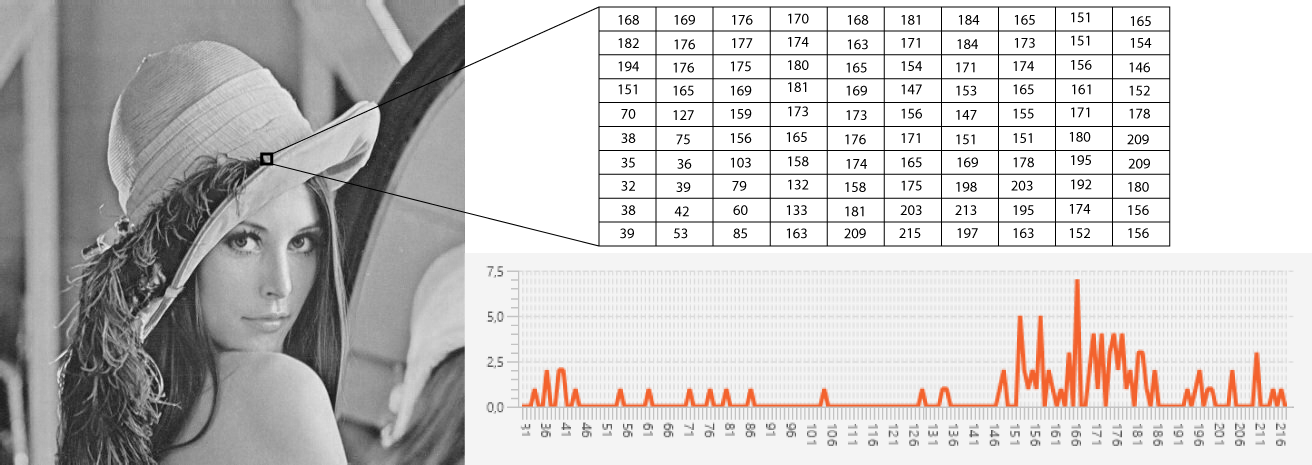
\includegraphics[width=1\textwidth]{imagens/histograma.png}
\label{fig:histograma}
\sourceAuthor
\end{figure}


Segundo \citet{conciAzevedoLeta:2008}, o histograma pode ser obtido da seguinte forma: analisa-se o tom de cada pixel; realiza-se a contagem do número de pixeis de cada intensidade de cor; representa-se esses valores na forma gráfica, correspondendo a frequência de cada tom.

Um processo comumente aplicado em técnicas de PDI é a convolução. Segundo \citet{pedriniSchwartz:2008}, o processo de convolução faz uso de matrizes, que são denominadas máscaras, para aplicar modificações na imagem pixel a pixel. A máscara, também conhecida como \textit{kernel} é uma matriz bidimensional quadrada. Usualmente, esta matriz possui um tamanho ímpar e dimensões quadradas, estas características são importantes para que a máscara possua um pixel central.

O processo de convolução utiliza os coeficientes desta máscaras para realizar uma multiplicação pelos níveis de cor dos pixeis. O pixel central é modificado pela média de todas as multiplicações. Este processo percorre a imagem aplicando a máscara em todos os pixel da imagem. Outro processo semelhante é o processo de correlação, onde este possui o mesmo princípio da convolução, mas com a diferença da máscara ser rotacionada em 180º \cite{gonzalesWoods:2008}. A implementação em java para o algoritmo pode ser acessado através do link: \url{https://bit.ly/2KJBGzc}.

Neste capítulo serão apresentadas algumas das principais técnicas de PDI. Dentre elas estarão limiarização, transformações geométricas, filtro de passa baixa e passa alta, morfologia matemática, afinamento e técnicas de classificação.
% ---
\section{Limiarização}
\label{sec:limiarizacao}

Limiarização ou \textit{Threshold} é uma técnica que consiste em comparar cada pixel da imagem com um \textit{Threshold} e a partir deste, gerar um novo valor para o pixel em processamento. Esta técnica tem como objetivo separar objetos da imagem que correspondem a um determinado nível de intensidade. Desta forma, esta técnica permite que, em uma imagem composta por objetos claros e com fundo escuro, os objetos desta imagem possam ser facilmente extraídos aplicando um \textit{threshold} com intensidade entre a cor de fundo e a cor dos objetos \cite{gonzalesWoods:2008}. A Figura \ref{fig:limiarizacaofig} exemplifica este procedimento.

\begin{figure}[ht]
\centering

\caption{\textbf{Imagem colorida (a) e a imagem correspondente após a aplicação do threshold}}
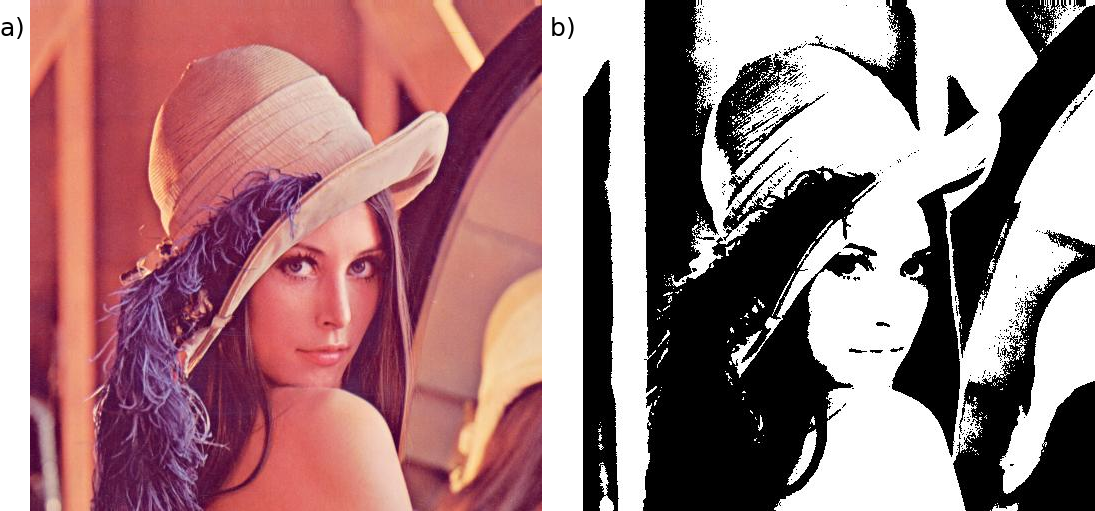
\includegraphics[width=0.6\textwidth]{imagens/limiarizacao.png}
\sourceAuthor
\label{fig:limiarizacaofig}
\end{figure}

Na Figura \ref{fig:limiarizacaofig} é aplicado um \textit{Threshold} de 190, desta forma, os pixels com valores maiores que 190 recebem a cor branca, enquanto os pixels com valores inferiores recebem a cor preta. A imagem resultante será composta por pixels pretos e brancos variando, sendo 0 ou 255.A implementação em java para o algoritmo pode ser acessado através do link: \url{https://bit.ly/2K1QO9S}

Uma maneira comum para a identificação do \textit{Threshold} a ser utilizado é através do histograma da imagem, sendo que através do histograma se tem uma visão geral da distribuição das tonalidades da imagem. Em um histograma com dois picos, o valor entre os dois picos pode ser utilizado como \textit{Threshold}, onde os picos representam as cores com maior ocorrência \cite{gonzalesWoods:2008}. 

% ---
\section{Brilho e Contraste}
O conceito de brilho está relacionado com a intensidade luminosa de uma fonte, quando é trabalhado com imagens digitais. Esta intensidade está relacionada com os pixels da imagem. O contraste está relacionado com a medida de variação da intensidade luminosa por unidade de área \cite{gonzalesWoods:2008}.

O brilho e contraste podem ser definidos através de uma função matemática. Esta função é definida por \(g = \alpha.f + \beta\), onde o \(g\) é o pixel resultante, \(\alpha\) é o coeficiente de contraste e \(\beta\) é o coeficiente de brilho e \(f\) é o pixel analisado \cite{pedriniSchwartz:2008}.

\begin{figure}[ht]
\centering
\caption{\textbf{Imagem colorida (a) e as imagens correspondentes após a aplicação de contraste com diferentes valores (b) e (c)}}
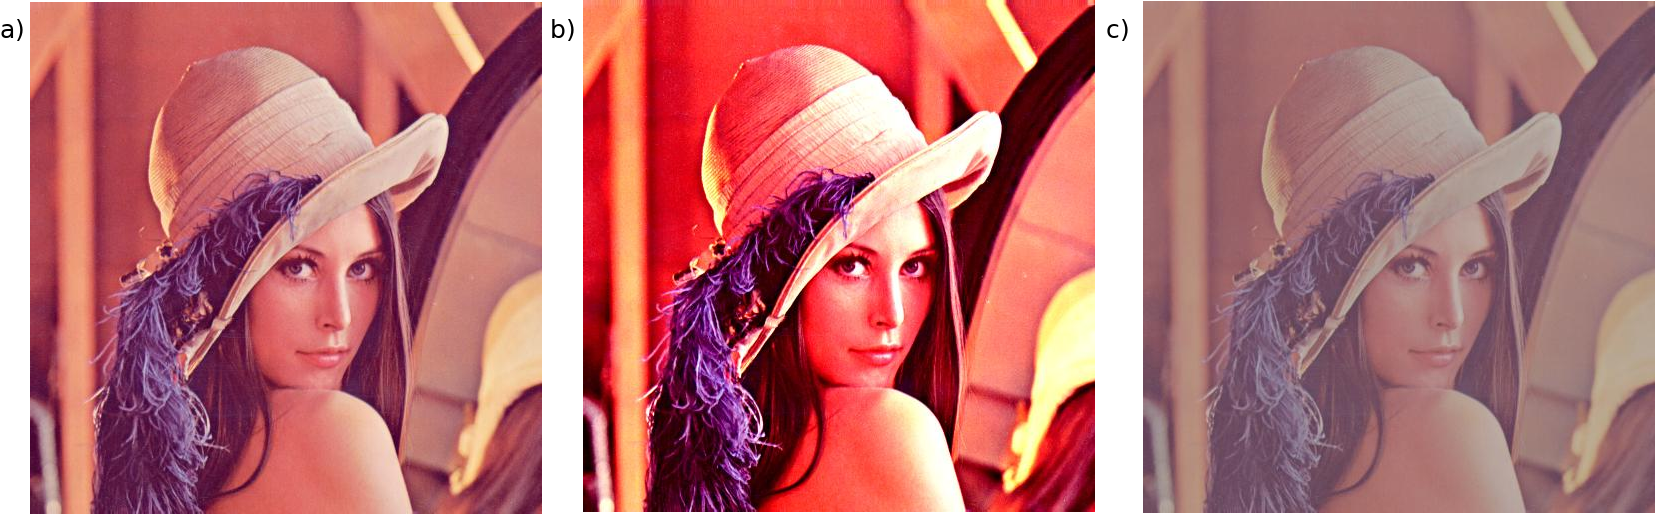
\includegraphics[width=0.9\textwidth]{imagens/contraste.png}
\sourceAuthor
\label{fig:contraste}
\end{figure}

A Figura \ref{fig:contraste} apresenta figuras que representam a imagem original (esquerda), o resultado após a aplicação de contraste utilizando o coeficiente 2 (b) e o resultado após a aplicação de contraste utilizando o coeficiente 0,5, respectivamente (c). A implementação em java para o algoritmo pode ser acessado através do link: \url{https://bit.ly/2JY8Dqj}

\begin{figure}[ht]
\centering
\caption{\textbf{Imagem colorida e a imagens correspondentes após a aplicação de brilho}}
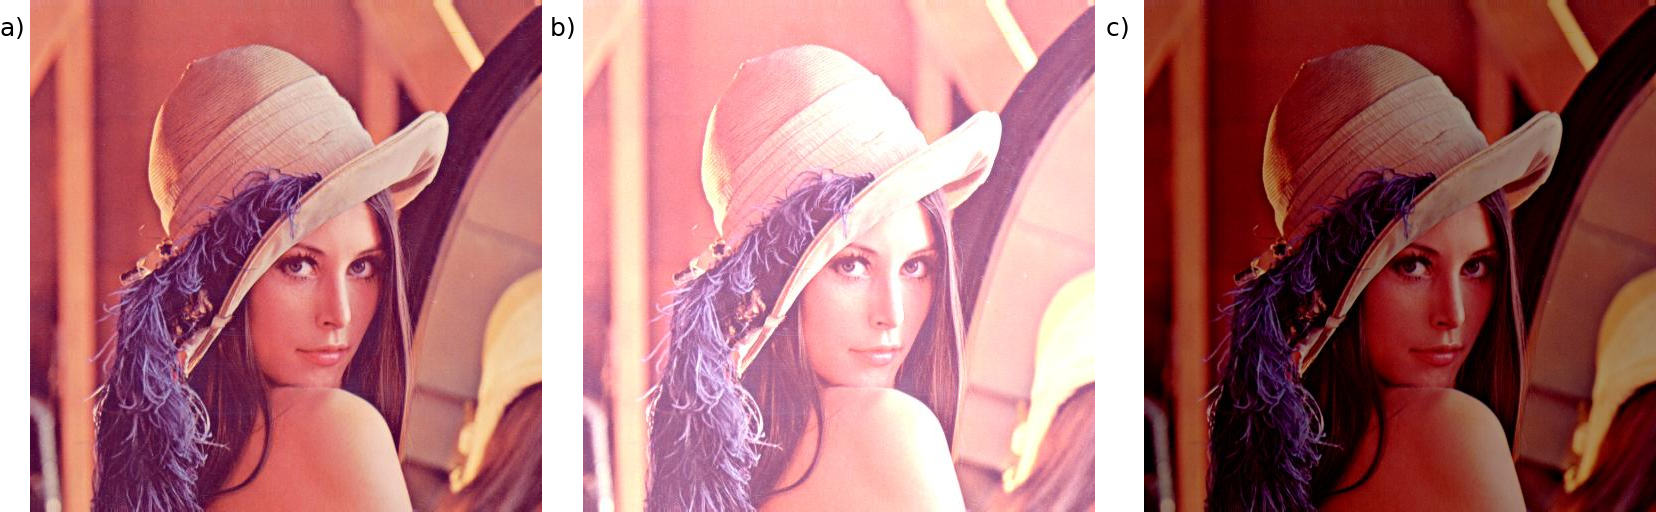
\includegraphics[width=0.9\textwidth]{imagens/brilho.png}
\sourceAuthor
\label{fig:brilho}
\end{figure}

A Figura \ref{fig:brilho} apresenta imagens que representam a imagem original (direita), o resultado após a aplicação de brilho utilizando o coeficiente 50 (b) e o resultado após a aplicação de brilho utilizando o coeficiente -50, respectivamente (c). A implementação em java para o algoritmo pode ser acessado através do link: \url{https://bit.ly/2FTWGPN}

% ---
\section{Transformações geométricas}

Transformações geométricas são aquelas que possuem o objetivo de permitir o mapeamento entre posições espaciais da imagem e a imagem modificada. Estas transformações consistem em aplicar operações responsáveis pela reorganização dos pixels da imagem \cite{pedriniSchwartz:2008}. São operações que modificam os tons dos pixel na posição (\(x_o, y_o\)) da imagem de origem para outra imagem (\(x_d, y_d\))de destino, alterando, desta forma, a posição dos pixels \cite{conciAzevedoLeta:2008}.

Transformações espaciais podem ser realizadas através da multiplicação de matrizes, expressa por:

\[
\begin{bmatrix}
    X’       \\ 
	Y’       \\ 
	Z’       \\ 
    1        \\ 
\end{bmatrix}
=
\begin{bmatrix}
    t_{11} & t_{12} & t_{13} & t_{14}   \\ 
	t_{21} & t_{22} & t_{23} & t_{24}   \\ 
	t_{31} & t_{32} & t_{33} & t_{34}   \\ 
	t_{41} & t_{42} & t_{43} & t_{44}   \\ 
\end{bmatrix}
.
\begin{bmatrix}
    X       \\ 
	Y       \\ 
	Z       \\ 
    1       \\ 
\end{bmatrix}
\]

Os valores X’, Y’, Z representam as coordenadas da imagem de destino que receberão o pixel analisado das coordenadas X, Y, Z da imagem de origem. Os valores \(t_x\), representam a matriz de transformação que deve ser aplicada para o pixel em análise.

% ---
\subsection{Translação}

O processo de transladar um objeto consiste em deslocar ou somar a cada um dos pixels da imagem um determinado valor (\(tx, ty, tz\)) \cite{conciAzevedoLeta:2008}. Segundo \citet{pedriniSchwartz:2008}, a translação de uma imagem, utilizando o deslocamento \(tx\), \(ty\) e \(tz\), pode ser expressa na forma matricial por:

\[
T
\begin{bmatrix}
    1 & 0 & 0 & t_x   \\ 
    1 & 0 & 1 & t_y   \\    
    0 & 0 & 1 & t_z   \\    
    0 & 0 & 0 & 1   \\  
\end{bmatrix} 
\]

A implementação em java para o algoritmo pode ser acessado através do link: \url{https://bit.ly/2KHJ26c}

% ---
\subsection{Mudança de escala}

O processo de mudança de escala (zoom in, zoom out) consiste na multiplicação de cada um dos pixels da imagem por um uma escala (\(s_x\), \(s_y\), \(s_z\))  \cite{conciAzevedoLeta:2008}. Segundo \citet{pedriniSchwartz:2008}, a mudança de escala de uma imagem, utilizando os fatores \(s_x\), \(s_y\) e \(s_z\), pode ser expressa na forma matricial por:

\[
T
\begin{bmatrix}
    1 & 0 & 0 & t_x   \\ 
	1 & 0 & 1 & t_y   \\ 
	0 & 0 & 1 & t_z   \\ 
	0 & 0 & 0 & 1     \\ 
\end{bmatrix} 
\]

A implementação em java para o algoritmo pode ser acessado através do link: \url{https://bit.ly/2IpuvxP}

% ---
\subsection{Reflexão}

A operação de reflexão ou espelhamento é uma operação que combina operações de rotação múltiplas do ângulo de 90º com uma inversão de coordenadas \cite{conciAzevedoLeta:2008}. Segundo \citet{pedriniSchwartz:2008}, operações de reflexão podem ser expressas na forma matricial por:

\[
E_{yz}
\begin{bmatrix}
    -1 & 0 & 0 & 0   \\ 
	 0 & 1 & 0 & 0   \\ 
	 0 & 0 & 1 & 0   \\ 
	 0 & 0 & 0 & 1   \\ 
\end{bmatrix} 
E_{xz}
\begin{bmatrix}
    0 &  0 & 0 & 0   \\ 
	0 & -1 & 0 & 0   \\ 
	0 &  0 & 1 & 0   \\ 
	0 &  0 & 0 & 1   \\ 
\end{bmatrix} 
E_{xy}
\begin{bmatrix}
    0 & 0 &  0 & 0   \\ 
	0 & 1 &  0 & 0   \\ 
	0 & 0 & -1 & 0   \\ 
	0 & 0 &  0 & 1   \\ 
\end{bmatrix} 
\]

Onde \(E_yz\) refere-se a reflexão no eixo \(xy\), \(E_xz\) refere-se a reflexão no eixo \(xz\) e \(E_xy\) refere-se a reflexão no eixo \(xy\).

Segundo \citet{conciAzevedoLeta:2008}, um \textit{flip} horizontal pode ser definido por uma rotação de 180º com os valores das coordenadas \(y_0\) invertidas (representado pela máscara \(E_yz\)) e um \textit{flip} vertical pode ser definido por uma rotação de 180º com os valores das coordenadas x0invertidas (representado pela máscara \(E_xz\));

A implementação em java para o algoritmo pode ser acessado através do link: \url{https://bit.ly/2KIZRxn}

% ---
\subsection{Rotação}

Segundo \citet{pedriniSchwartz:2008}, a operação de rotação pode ser realizada aplicando a rotação de um ponto em cada eixo de coordenadas. A rotação de um ponto em torno do eixo x utilizando um ângulo \(\alpha\), pode ser descrita por:

\[
R_\alpha
\begin{bmatrix}
    1 &         0 &          0 & 0   \\ 
	0 & cos\alpha & -sen\alpha & 0   \\ 
	0 & sen\alpha &  cos\alpha & 0   \\ 
	0 &         0 &          0 & 1   \\ 
\end{bmatrix} 
\]

A rotação de um ponto em torno do eixo y utilizando um ângulo \(\beta\), pode ser descrita por:

\[
R_\beta
\begin{bmatrix}
     cos\beta & 0 & sen\beta & 0   \\ 
	        0 & 1 & 0        & 0   \\ 
	-sen\beta & 0 & cos\beta & 0   \\ 
            0 & 0 &        0 & 1   \\ 
\end{bmatrix} 
\]

A rotação de um ponto em torno do eixo z utilizando um ângulo \(\gamma\), pode ser descrita por:

\[
R_\gamma
\begin{bmatrix}
    cos\gamma & -sen\gamma & 0 & 0   \\ 
	sen\gamma &  cos\gamma & 0 & 0   \\ 
	        0 &          0 & 1 & 0   \\ 
            0 &          0 & 0 & 1   \\ 
\end{bmatrix} 
\]

A implementação em java para o algoritmo pode ser acessado através do link: \url{https://bit.ly/2I4hQga}

\begin{figure}[ht]
\centering
\caption{\textbf{Aplicação de filtros de transformações geométricas em uma imagem}}
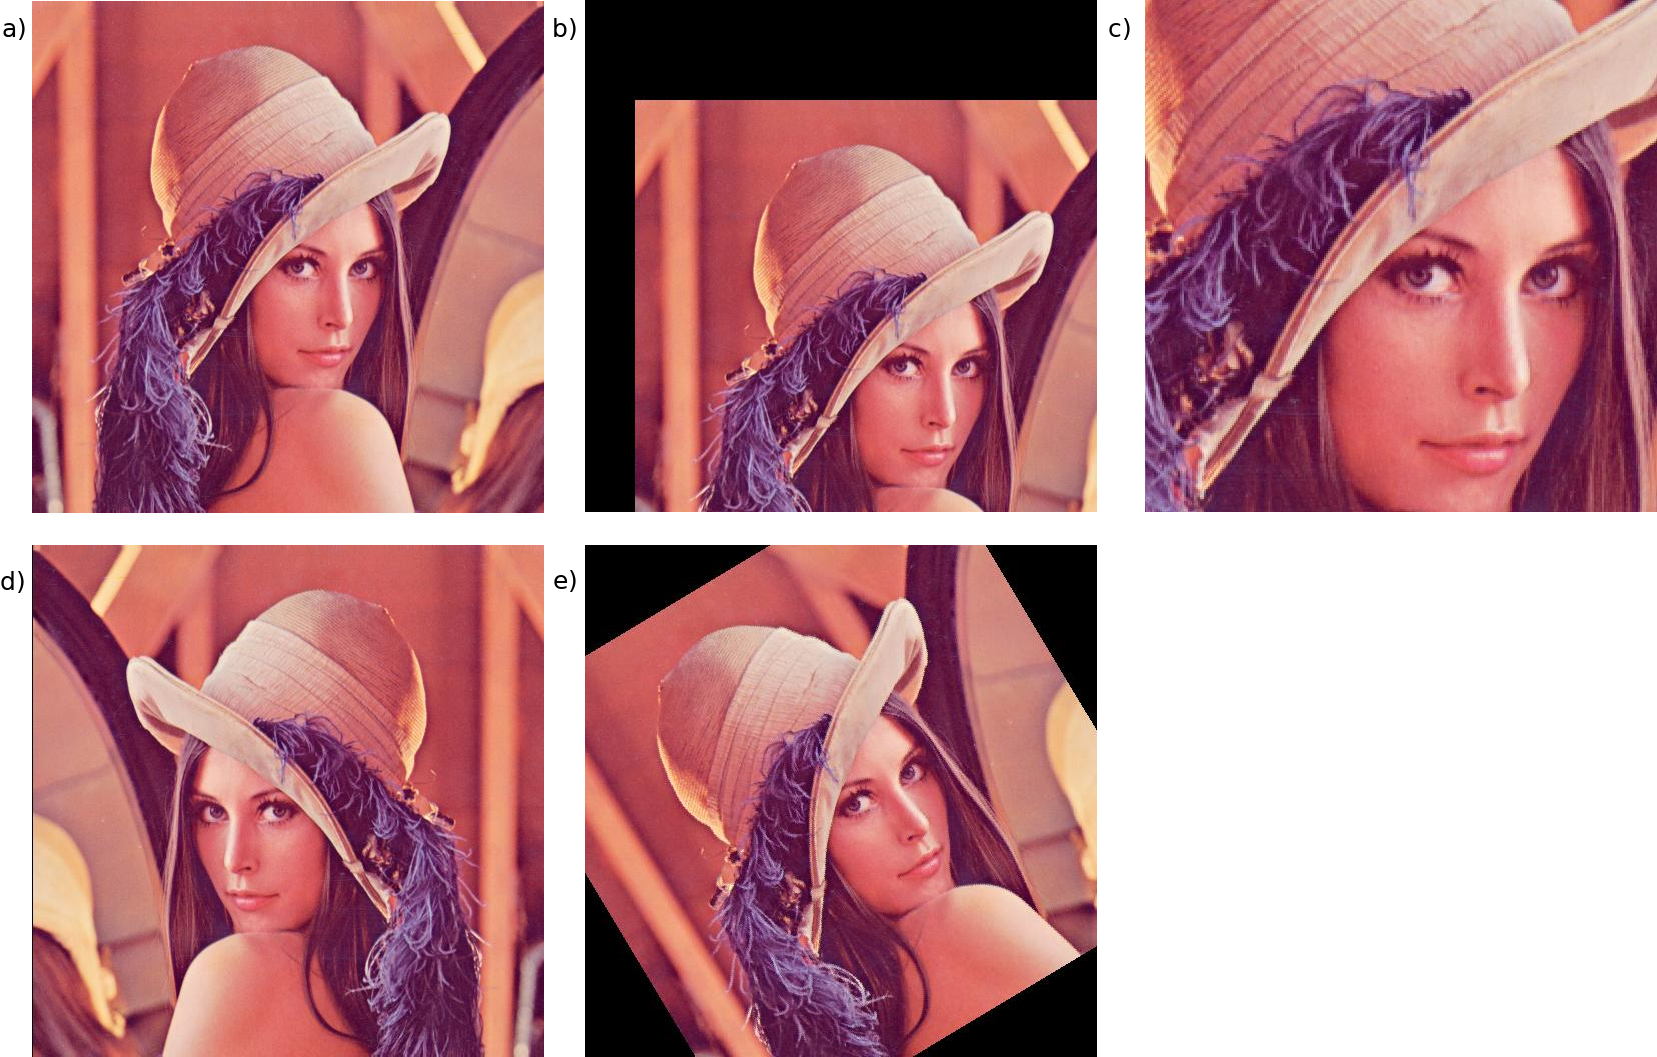
\includegraphics[width=0.9\textwidth]{imagens/transformacoesgeometricas.png}
\sourceAuthor
\label{fig:transformacoesgeometricas}
\end{figure}

Na Figura \ref{fig:transformacoesgeometricas} é apresentada a aplicação de transformações geométricas. O primeiro processo apresentado é a translação (b), onde a imagem original é transladada em 50 pixels no \(eixo x\) e 100 pixels no \(eixo y\). Sequencialmente é apresentado a imagem original (a), o processo de mudança de escala utilizando o valor o fator 2 (c), a reflexão horizontalmente (d) e a rotação da imagem (e). 

% ---
\section{Filtros passa baixa (Suavização)}
Filtros do tipo passa baixa são aqueles utilizados para a extração e limpeza de imagens. Existem diversas técnicas que permitem esta operação e a escolha deve ser feita com base no tipo de imagem a ser analisada e na informação desejada desta. 

O efeito visual resultante da aplicação de um filtro passa baixa é o da suavização e redução das variações nos níveis de cinza da imagem. Sua aplicação tende a reduzir ruídos, mas como consequência, a imagem tende a perder nitidez \cite{conciAzevedoLeta:2008}.

% ---
\subsection{Média}
Filtros de média são utilizadas para fins de suavização de imagens, sendo utilizados para o borramento e a redução de ruídos. A ideia por trás desta técnica é aplicar uma operação estatística na vizinhança de uma máscara, calculando um novo valor do pixel analisado \cite{gonzalesWoods:2008}. 

O filtro de média calcula a média aritmética da máscara em processamento, o valor resultante será aplicado no pixel central. Este filtro diminui variações da imagem, removendo, desta forma, seu ruído desta \cite{gonzalesWoods:2008}.

A implementação em java para o algoritmo pode ser acessado através do link: \url{https://bit.ly/2jGc7CM} 

% ---
\subsection{Moda}
O filtro de moda calcula o ponto de maior frequência entre os da área em processamento. É indicado para a remoção de ruídos aleatoriamente distribuídos como o ruído gaussiano ou o uniforme \cite{gonzalesWoods:2008}. Neste filtro, os valores existentes na máscara são ordenado e é utilizado o como novo valor o valor mais frequente \cite{conciAzevedoLeta:2008}.

A implementação em java para o algoritmo pode ser acessado através do link: \url{https://bit.ly/2Io3U46}

% ---
\subsection{Mediana}

O filtro de mediana é o filtro estatístico mais conhecido, onde substitui o valor de um determinado pixel pela mediana dos níveis de intensidade da vizinhança. Este tipo de filtro é utilizado quando se deseja reduzir ruídos aleatórios de uma imagem. O filtro propicia um menor borramento do que filtros lineares de suavização como o filtro de média \cite{gonzalesWoods:2008}.

A mediana \(m\) de um conjunto contendo um número \(n\) de elementos é definida pelo valor central destes elementos, desta forma, a metade dos elementos situam-se acima de \(m\) e a outra metade abaixo. Quando \(n\) for par, é necessário realizar a média aritmética dos elementos mais próximos aos centro \cite{conciAzevedoLeta:2008}.

Este filtro realiza a ordenação das intensidades dos pixels existentes dentro da máscara, utilizando como valor para o pixel analizado o valor central dos elementos ordenados \cite{conciAzevedoLeta:2008}.

O filtro de mediana possui resultados melhores do que o filtro de média. Isso ocorre devido ao fato de que, se existe um ruído entre os elementos da máscara, este valor estará presente nas primeiras ou últimas posições. Desta forma, pontos discrepantes têm grande chance de serem considerados ruídos e suavizados \cite{conciAzevedoLeta:2008}.

A implementação em java para o algoritmo pode ser acessado através do link: \url{https://bit.ly/2wi5EXL} 

% ---
\subsection{Filtro Gaussiano}
Filtros Gaussianos possuem características que são úteis para o processamento de imagens. As funções Gaussianas são simétricas, o que significa que o grau de suavização é aplicado da mesma forma em todas as direções (isotrópico). A suavização da imagem é obtida através da substituição de cada pixel da imagem pela média ponderada dos pixels vizinhos \cite{pedriniSchwartz:2008}. 

Este filtro é utilizado para reduzir quantidades de variação de intensidades entre o pixel e seus vizinhos, minimizando e até eliminado informações indesejadas. É um dos filtros de passa-baixa mais importantes, pois seu nível de suavização ocorre de maneira uniforme, o que não ocorre nos outros filtros, como, por exemplo, no filtro de média. Este filtro é adequado para a aplicação em conjunto com outros filtros em aplicações de detecção de bordas \cite{conciAzevedoLeta:2008}.   

Segundo \citet{pedriniSchwartz:2008}, em filtros Gaussianos, os coeficientes da máscara de processamento são obtidos através de uma função Gaussiana bidimensional. A função Gaussiana com média zero e desvio padrão \(\sigma\) é descrita por:

\begin{figure}[ht]
\centering
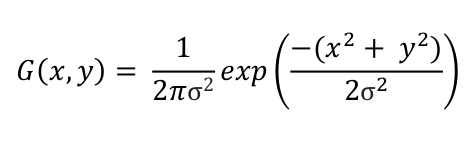
\includegraphics[width=0.8\textwidth]{imagens/gauss_formula.png}
\end{figure}

A aplicação de um filtro Gaussiano pode ser realizada através de convoluções por meio de matrizes. Abaixo são descritas duas máscaras para este filtro, ambas com \(\sigma\) = 0.

\begin{figure}[ht]
\centering
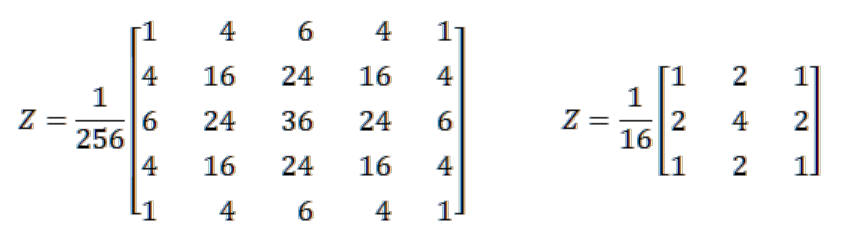
\includegraphics[width=0.8\textwidth]{imagens/gauss_mascara.png}
\end{figure}

A implementação em java para o algoritmo pode ser acessado através do link: \url{https://bit.ly/2KIrx5F}

\begin{figure}[ht]
\centering
\caption{\textbf{Aplicação de filtro passa baixa em uma imagem}}
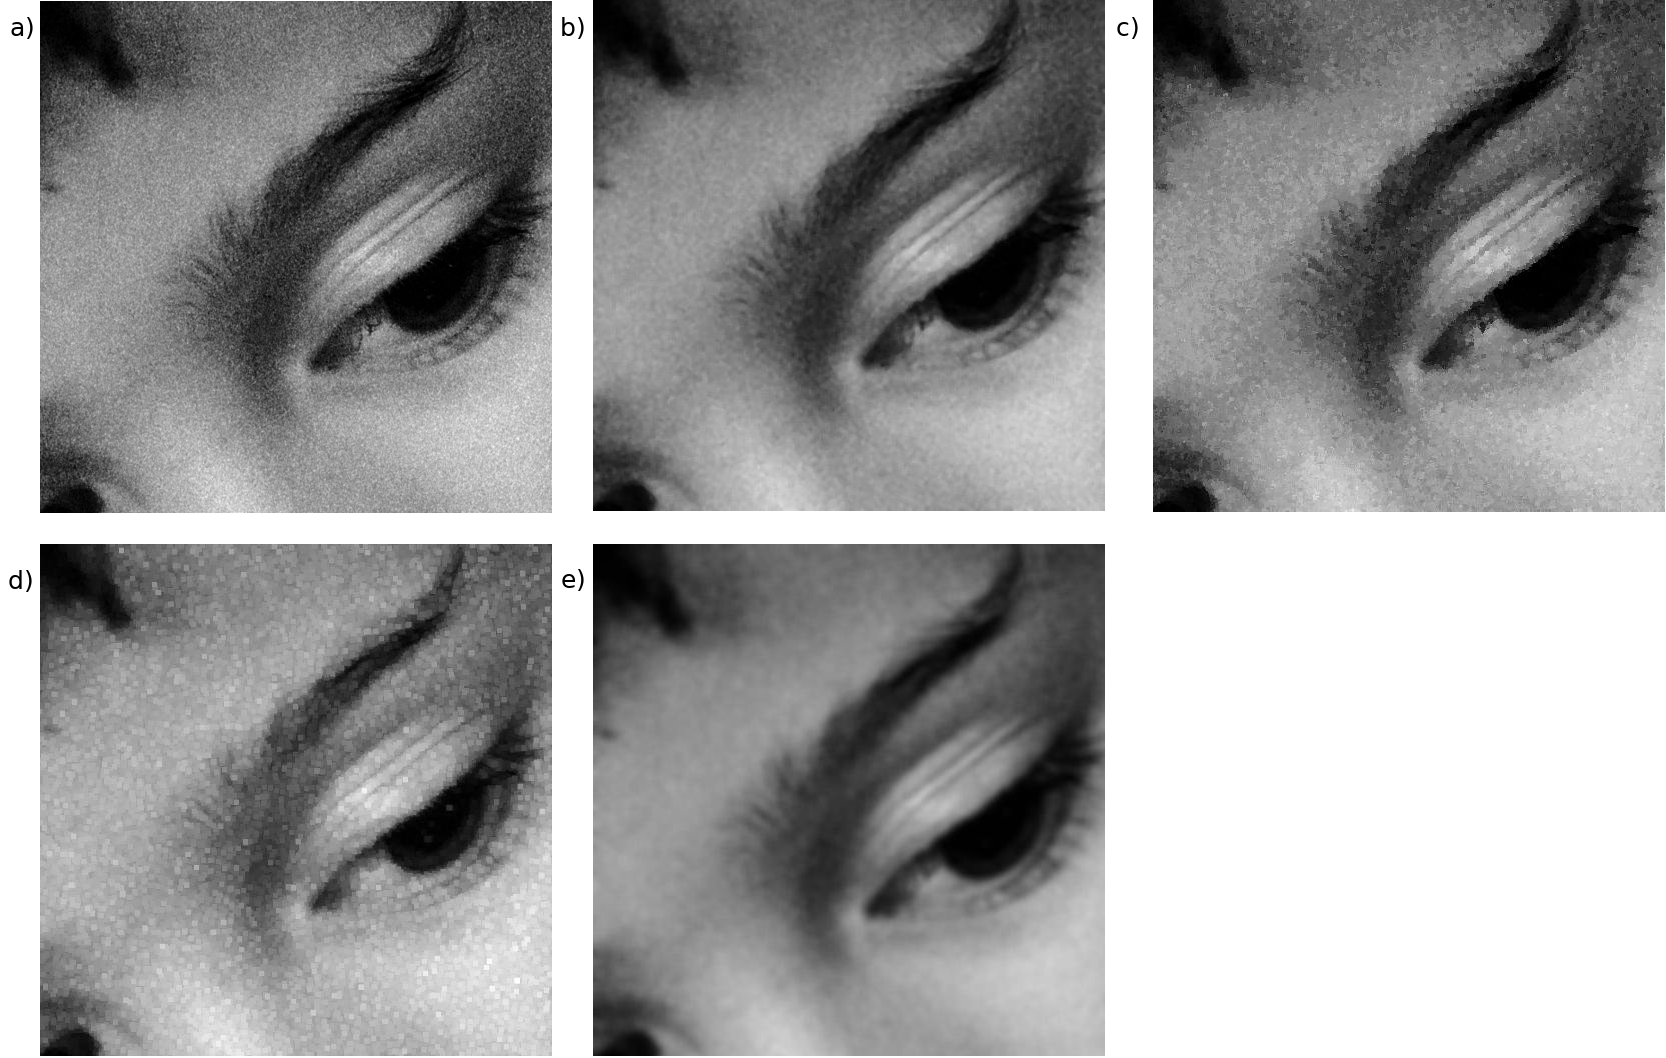
\includegraphics[width=0.9\textwidth]{imagens/suavizacao.png}
\sourceAuthor
\label{fig:suavizacao}
\end{figure}

Na Figura \ref{fig:suavizacao} é apresentado um conjunto de aplicações de filtros passa baixa para a suavização da imagem de origem. A imagem (a) representa a imagem original.  O primeiro filtro apresentado é o filtro da média (b), seguido do filtro moda (c), mediana (d) e o filtro Gaussiano (e).

% ---
\section{Filtros passa-alta}

Filtros passa-alta diminuem ou eliminam baixas frequências, realçando as altas frequências. São filtros que destacam características como bordas, linhas e curvas, indicado mudanças repentinas nos níveis de intensidade entre duas regiões. Em geral, o resultado obtido através destes filtros é o de tornar mais nítidas as transições entre regiões da imagem \cite{conciAzevedoLeta:2008}.

Segundo \citet{pedriniSchwartz:2008}, técnicas de detecção de bordas fazem uso de uma abordagem onde é realizado um cálculo de um operador local, que determina uma mudança abrupta de níveis de cinza. Uma borda é uma fronteira ou limite entre regiões com intensidades distintas de níveis de cinza

Um operador utilizado para a detecção de mudanças significativas nos níveis de cinza de uma imagem é o gradiente. O gradiente é um vetor cuja direção indica os locais onde os níveis de cinza sofreram maior variação \cite{pedriniSchwartz:2008}. Técnicas de detecção de contornos assumem que a transição entre regiões a serem segmentadas são caracterizadas por um variação nos níveis de cinza da imagem, desta forma, uma grande variação dos níveis de cinza pode indicar a presença das fronteiras entre objetos \cite{conciAzevedoLeta:2008}. 

O gradiente de uma imagem, para a função \(f(x,y)\) na coordenadas \(x,y\), pode ser definido como um vetor formado pelas suas derivadas parciais:

\begin{figure}[ht]
\centering
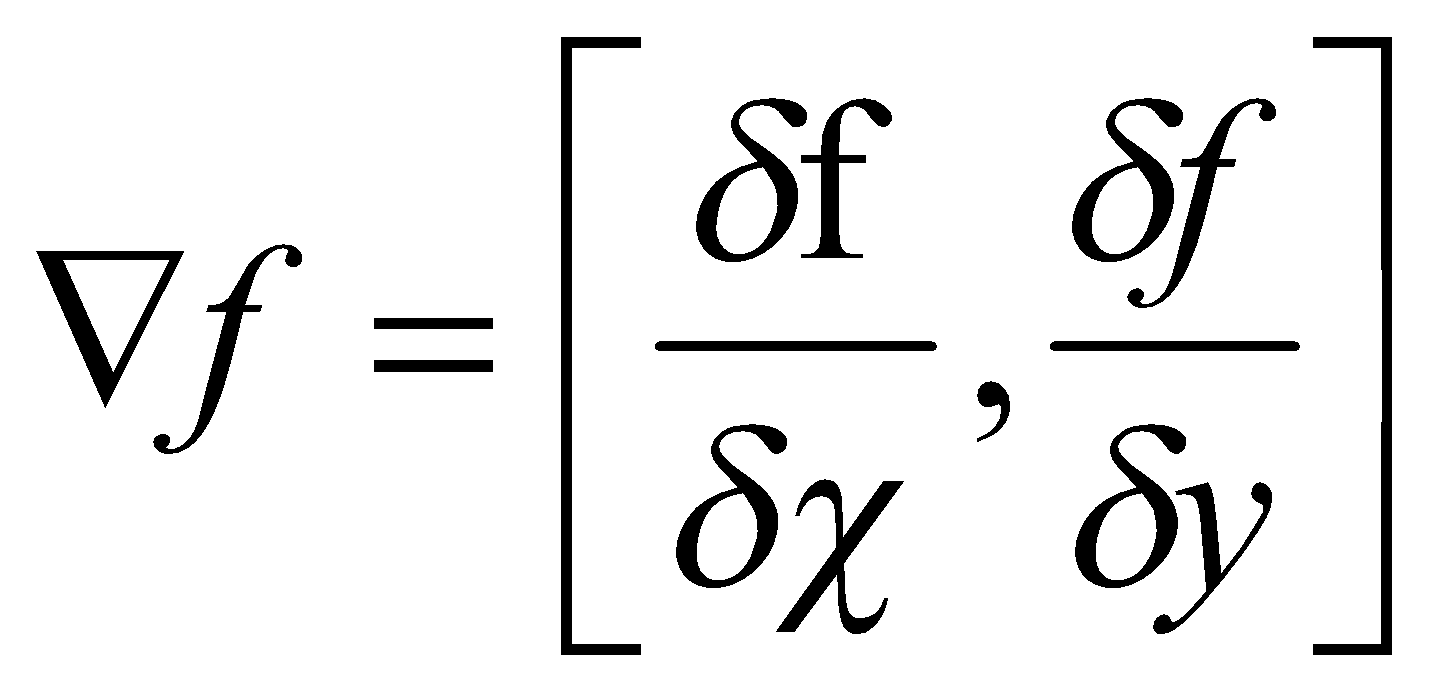
\includegraphics[width=0.3\textwidth]{imagens/gradiente.png}

Equação 1.1
\end{figure}

A magnitude do gradiente se relaciona com a taxa de variação da imagem por unidade de distância. Este valor pode ser definido através da fórmula abaixo:

\begin{figure}[ht]
\centering
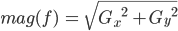
\includegraphics[width=0.4\textwidth]{imagens/magnitude.png}
\end{figure}


Onde \(G_x\) e \(G_y\) corresponde ao resultado da multiplicação da matriz Z, que corresponde aos tons da região analisada, com as máscaras de convolução \(G_x\) e \(G_y\) respectivamente


\[
Z
\begin{bmatrix}
    z_0 & z_1 & z_2   
	z_3 & z_4 & z_5      
	z_6 & z_7 & z_8      
\end{bmatrix} 
\]

% ---
\subsection{Sobel}

O operador de Sobel realiza a aproximação da magnitude do gradiente através da diferença de valores ponderados dos níveis de cinza da imagem. Para isso, são utilizados duas máscaras de tamanho 3 x 3, sendo que uma é aplicada em relação ao \(eixo\) \(x\) e a outro é aplicada no \(eixo\) \(y\) \cite{pedriniSchwartz:2008}. Este operador realiza um suavização, e ao mesmo tempo, o realce de bordas.

\[
G_x
\begin{bmatrix}
    -1 & 0 & 1   \\ 
	-2 & 0 & 1   \\ 
	-1 & 0 & 1   \\ 
\end{bmatrix} 
G_y
\begin{bmatrix}
    -1 & -2 & -1   \\ \hline
	 0 &  0 & 0    \\ \hline   
	 1 &  2 & 1    \\ \hline   
\end{bmatrix} 
\]

Considerando \(z_0\) a \(z_8\) os tons de cinza em torno do pixel que está sendo analisado, este filtro é definido pela equação (Equação 1.1) onde:

\[Gx = (z_6 + 2z_7 + z_8) - (z_0 + 2z_1 + z_2)\]
\[Gy = (z_2 + 2z_5 + z_8) - (z_0 + 2z_3 + z_6)\]

A implementação em java para o algoritmo pode ser acessado através do link: \url{https://bit.ly/2HYVgcU}

% ---
\subsection{Roberts}
O operador de Roberts corresponde ao método mais simples de detecção de bordas. Como resultado, em regiões que possuem contraste bem definido, obtém-se uma imagem com intensidades altas, e baixos valores em regiões com pouco contraste. Este operador caracteriza-se por um orientação a 45º, desta forma, bordas inclinadas são mais realçadas que outras. Outra característica deste operador é a sensibilidade a ruído \cite{conciAzevedoLeta:2008}.

O operador de Roberts faz uso de duas máscaras de tamanho 2 x 2, sendo que uma é aplicada no sentido horizontal e a outro é aplicada no sentido vertical \cite{pedriniSchwartz:2008}.


\[
G_x
\begin{bmatrix}
    1 &  0    \\ 
	0 & -1    \\    
\end{bmatrix} 
G_y
\begin{bmatrix}
    0 & -1   \\ 
	1 &  0   \\    
\end{bmatrix} 
\]

Considerando \(z_0\) a \(z_8\) os tons de cinza em torno do pixel que está sendo analisado, este filtro é definido por (Equação 1.1):

\[G_x = z_0 - z_4\]
\[G_y = z_3 -z_1\]

A implementação em java para o algoritmo pode ser acessado através do link: \url{https://bit.ly/2KIsb35}
% ---
\subsection{Prewith}

O operador de Prewith faz uso de duas máscaras de tamanho 3 x 3, sendo que uma é aplicada no sentido horizontal e a outro é aplicada no sentido vertical \cite{pedriniSchwartz:2008}.	

\[
G_x
\begin{bmatrix}
    -1 & 0 & 1   \\ 
	-1 & 0 & 1   \\ 
	-1 & 0 & 1   \\    
\end{bmatrix} 
G_y
\begin{bmatrix}
    -1 & -1 & -1   \\ 
	 0 &  0 &  0   \\ 
	 1 &  1 &  1   \\    
\end{bmatrix} 
\]

Este filtro faz uso do mesmo conceito de Sobel e Roberts. Considerando \(z0\) a \(z8\) os tons de cinza em torno do pixel que está sendo analisado, este filtro é definido por:

\[Gx = (z_6 + z_7 + z_8) - (z_0 + z_1 + z_2)\]
\[Gy = (z_2 + z_5 + z_8) - (z_0 + z_3 + z_6)\]

A implementação em java para o algoritmo pode ser acessado através do link: \url{https://bit.ly/2wrt2lQ} 

% ---
\subsection{Kirsch}
O operador Kirsch (KIRSCH, 1971) consiste na utilização de oito máscaras orientadas em 45º. Para cada pixel da imagem é realizada a aplicação de uma das oito máscaras e é mantido o valor máximo. Desta forma, o gradiente não é obtido através dos valores de \(G_x\) e \(G_y\) separadamente, e sim, atrás do maior resultado do conjunto de 8 máscaras \cite{pedriniSchwartz:2008}.

\[
\begin{bmatrix}
     5 & -3 & -3   \\ 
	 5 &  0 & -3   \\ 
	 5 & -3 & -3   \\    
\end{bmatrix} 
\begin{bmatrix}
    -3 & -3 & -3   \\
	 5 &  0 & -3   \\
	 5 &  5 & -3   \\
\end{bmatrix}
\begin{bmatrix}
    -3 & -3 & -3   \\
	-3 &  0 & -3   \\
	 5 &  5 &  5   \\
\end{bmatrix} 
\begin{bmatrix}
    -3 & -3 & -3   \\
	-3 &  0 &  5   \\
	-3 &  5 &  5   \\
\end{bmatrix}
\]

\[
\begin{bmatrix}
    -3 & -3 &  5   \\ 
	-3 &  0 &  5   \\ 
	-3 & -3 &  5   \\ 
\end{bmatrix} 
\begin{bmatrix}
    -3 &  5 &  5   \\ 
	-3 &  0 &  5   \\ 
	-3 & -3 & -3   \\ 
\end{bmatrix}
\begin{bmatrix}
     5 &  5 &  5   \\ 
	-3 &  0 & -3   \\ 
	-3 & -3 & -3   \\ 
\end{bmatrix} 
\begin{bmatrix}
     5 &  5 & -3   \\ 
	 5 &  0 & -3   \\ 
	-3 & -3 & -3   \\ 
\end{bmatrix}
\]

Outras máscaras maiores podem ser aplicadas, como máscaras de tamanho 5 x 5 ou 7 x 7 pixel, mas estas abordagens são menos sensíveis a ruído e o tempo para a realização dos cálculos destas máscaras aumenta significamente \cite{pedriniSchwartz:2008}.

A implementação em java para o algoritmo pode ser acessado através do link: \url{https://bit.ly/2jG3HLs}

% ---
\subsection{Robinson}
Robson propôs um conjunto de oito máscaras onde a magnitude é calculada de maneira semelhante a realizada por Kirsh, ou seja, utilizando o valor máximo entre as oito máscaras \cite{pedriniSchwartz:2008}. 

\[
\begin{bmatrix}
     1 &  0 & -1   \\ 
	 2 &  0 & -2   \\ 
	 1 &  0 & -1   \\ 
\end{bmatrix} 
\begin{bmatrix}
     0 & -1 & -2   \\ 
	 1 &  0 & -1   \\ 
	 2 &  1 &  0   \\ 
\end{bmatrix}
\begin{bmatrix}
    -1 & -2 & -1   \\ 
	 0 &  0 &  0   \\ 
	 1 &  2 &  1   \\ 
\end{bmatrix} 
\begin{bmatrix}
    -2 & -1 &  0   \\ 
	-1 &  0 &  1   \\ 
	 0 &  1 &  2   \\ 
\end{bmatrix}
\]

\[
\begin{bmatrix}
    -1 & -0 &  1   \\ 
	-2 &  0 &  2   \\ 
	-1 &  0 &  1   \\ 
\end{bmatrix} 
\begin{bmatrix}
     0 &  1 &  2   \\ 
	-1 &  0 &  1   \\ 
	-2 & -1 &  0   \\ 
\end{bmatrix}
\begin{bmatrix}
     1 &  2 &  1   \\ 
	 0 &  0 &  0   \\ 
	-1 & -2 & -1   \\ 
\end{bmatrix} 
\begin{bmatrix}
     2 &  1 &  0   \\ 
	-1 &  0 & -1   \\ 
	-0 & -1 & -2   \\ 
\end{bmatrix}
\]

A implementação em java para o algoritmo pode ser acessado através do link: \url{https://bit.ly/2HWssSd}

% ---
\subsection{Frei-Chein}
O operador Frei-Chein utiliza um conjunto de nove máscaras de tamanho 3 x 3. As máscara M1 a M4 são utilizadas para realizar a detecção de bordas, já a M5 a M8 realizam a detecção de retas, e a M9 representa a média dos pixels na região da matriz \cite{pedriniSchwartz:2008}. 

\[
M1
\begin{bmatrix}
     	 	 	 1 &  \sqrt{2} &  1         \\ 
	             0 &         0 &  0         \\ 
	            -1 & -\sqrt{2} & -1         \\ 
\end{bmatrix} 
M2
\begin{bmatrix}
     	     0 &             1 & -1         \\ 
	  \sqrt{2} &             0 & -\sqrt{2}  \\ 
	         1 &             0 & -1         \\ 
\end{bmatrix}
M3
\begin{bmatrix}
     	 	 0 &            -1 & \sqrt{2}   \\ 
	         1 &             0 & -1         \\ 
	 -\sqrt{2} &             1 &  0         \\ 
\end{bmatrix} 
\]

\[
M4
\begin{bmatrix}
      \sqrt{2} &            -1 &  0         \\
	        -1 &             0 & 1          \\
	         0 &             1 & -\sqrt{2}  \\
\end{bmatrix} 
M5
\begin{bmatrix}
    	 	 0 &             1 &  0          \\ 
	        -1 &             0 & -1          \\ 
	         0 &             1 &  0          \\ 
\end{bmatrix}
M6
\begin{bmatrix}
  	 	 	-1 &             0 &  1          \\ 
             0 &             0 &  0          \\ 
             1 &             0 & -1          \\ 
\end{bmatrix} 
\]

\[
M7
\begin{bmatrix}
            1 &            -2 &  1           \\ 
	       -2 &             4 & -2           \\ 
	        1 &            -2 &  1           \\ 
\end{bmatrix} 
M8
\begin{bmatrix}
           -2 &             1 & -2            \\
	        1 &             4 &  1            \\
	       -2 &             1 & -2            \\
\end{bmatrix}
M9
\begin{bmatrix}
     	 	 1 &             1 &  1           \\
	         1 &             1 &  0           \\
	         1 &             1 & -1           \\
\end{bmatrix} 
\]

A implementação em java para o algoritmo pode ser acessado através do link: \url{https://bit.ly/2K227ig}

\begin{figure}[ht]
\centering
\caption{\textbf{Algoritmos de detecção de bordas}}
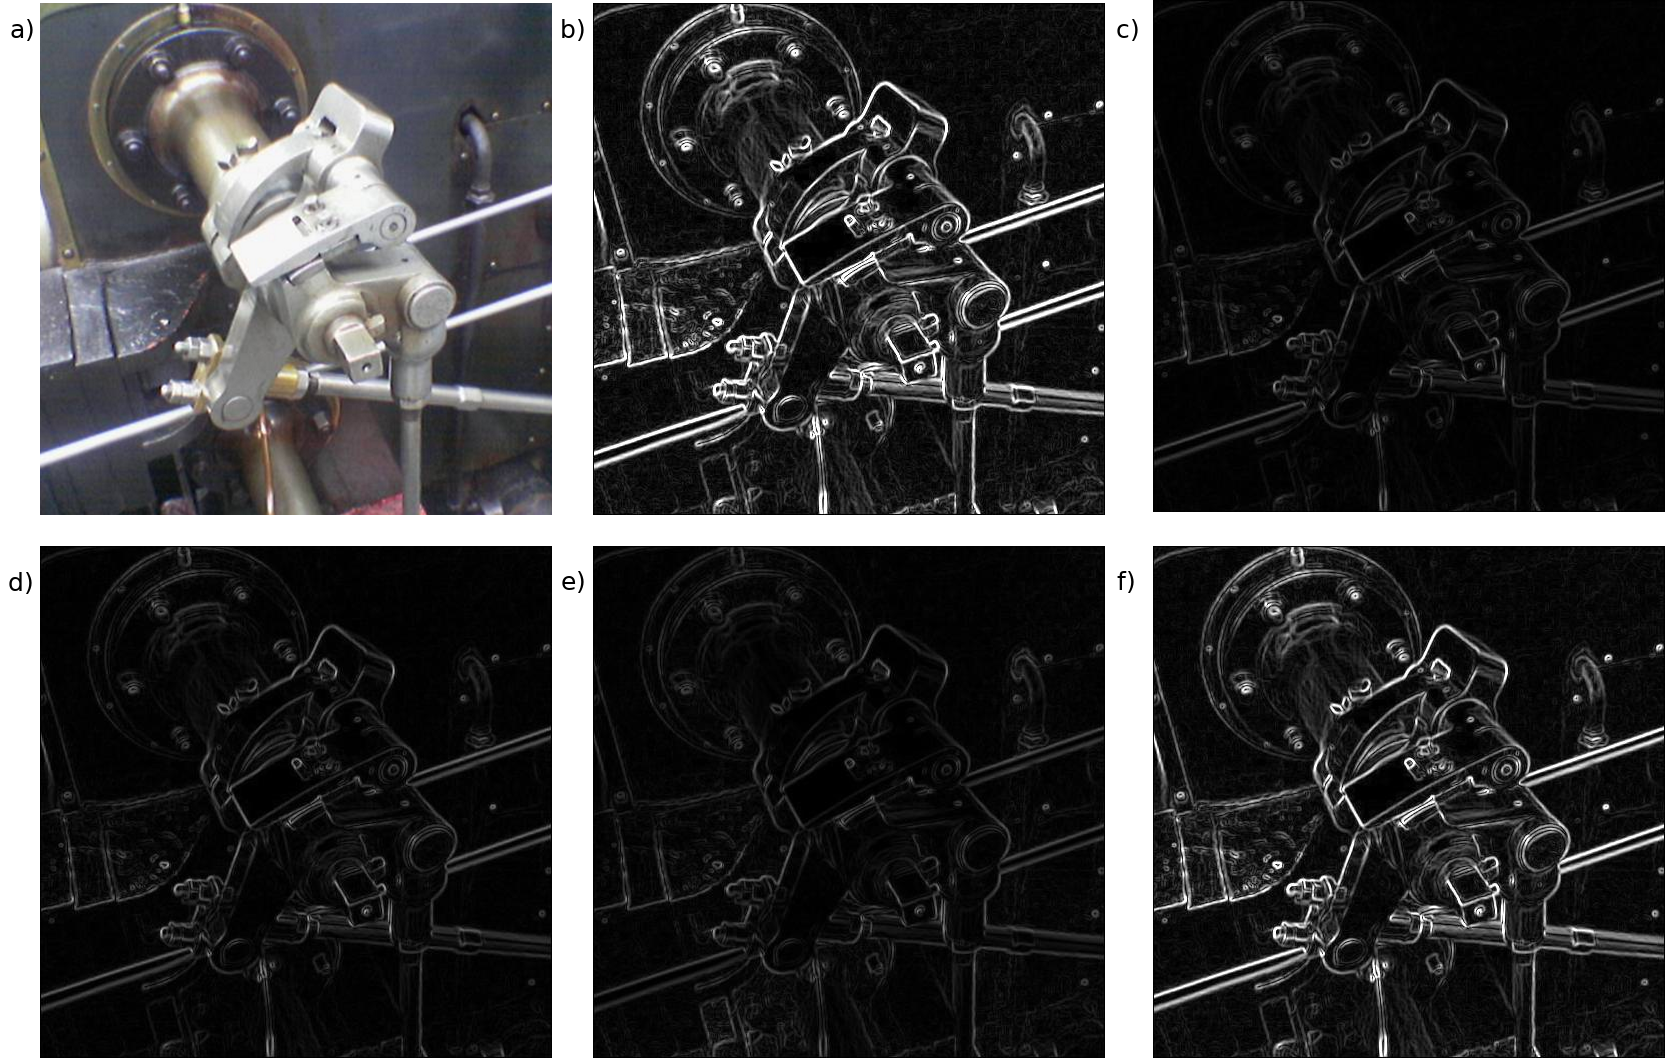
\includegraphics[width=0.9\textwidth]{imagens/deteccao_bordas.png}
\sourceAuthor
\label{fig:deteccao_bordas}
\end{figure}

A Figura \ref{fig:deteccao_bordas} apresenta o resultado da aplicação de detecção de bordas. A primeira imagem (a) representante a imagem original. O primeiro algoritmo é o Sobel (b), seguido de Kircsh (c), Robinson (d), Frei Chen (e) e Prewitt.

% ---
\subsection{Canny}

O operador de \citet{canny:1986} propõem um método que tem como objetivo otimizar a detecção de bordas em uma imagem que possui ruídos. Este método é o mais complexo, mas geralmente tem resultados superiores aos demais métodos com a mesma finalidade. Esta técnica é dividida em etapas. Inicialmente a imagem é suavizada através a aplicação de um filtro Gaussiano. Após esta suavização, são calculadas a magnitude e a direção do gradiente. Após o cálculo do gradiente, a borda é encontrada utilizando apenas os pontos onde a magnitude seja máxima na direção do gradiente, reduzindo assim, a espessura da borda \cite{pedriniSchwartz:2008}.

A após a identificação da borda, é possível que a imagem ainda contenha certos fragmentos causadores de ruído. Para solucionar este problema, o operador de \citet{canny:1986} faz uso de dois limiares \(T_1\) e \(T_2\), constituindo a etapa denominada limiarização com histerese. Desta forma, os pontos da borda que possuem gradiente maiores que \(T_2\) são mantidos na imagem. Pontos que estão conectados a estes pontos e que possuem magnitude de gradiente maior que T1 também são considerados como pertencentes a borda \cite{pedriniSchwartz:2008}.

A implementação em java para o algoritmo pode ser acessado através do link: \url{https://bit.ly/2jG3YxY}

% ---
\subsection{Marr and Hildreth}
Segundo \citet{pedriniSchwartz:2008}, o operador de Marr and Hildreth (MARR; HILDRETH, 1980) faz uso de uma máscara de tamanho 7 x 7 onde é realizado um processo de convolução. Esta matriz pode ser descrita por:

\[
H 
\begin{bmatrix}
     0 &  0 & -1 & -1 & -1 &  0 &  0            \\ 
     0 & -2 & -3 & -3 & -3 & -2 &  0            \\ 
    -1 & -3 &  5 &  5 &  5 & -3 & -1            \\ 
    -1 & -3 &  5 & 16 &  5 & -3 & -1            \\ 
    -1 & -3 &  5 &  5 &  5 & -3 & -1            \\ 
     0 & -2 & -3 & -3 & -3 & -2 &  0            \\ 
     0 &  0 & -1 & -1 & -1 &  0 &  0            \\ 
\end{bmatrix} 
\]

A implementação em java para o algoritmo pode ser acessado através do link: \url{https://bit.ly/2jDAeSp}

\begin{figure}[ht]
\centering
\caption{\textbf{Algoritmos de detecção de bordas de Canny e Marr and Hildreth}}
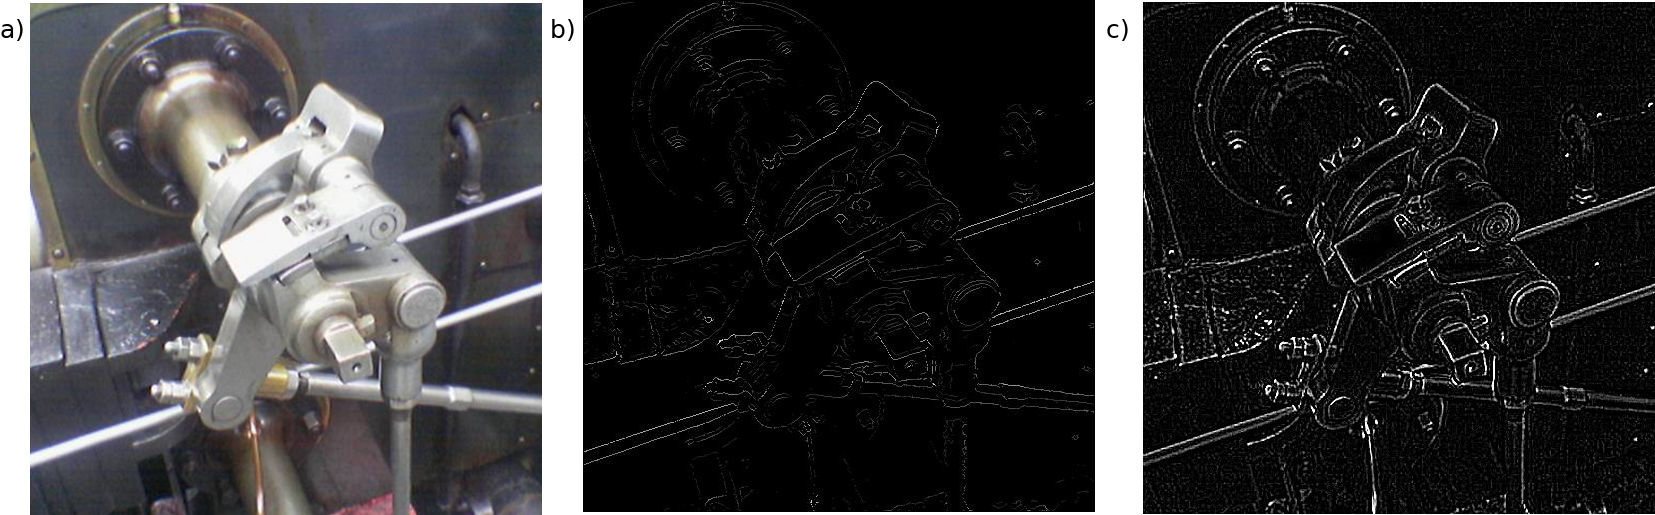
\includegraphics[width=0.9\textwidth]{imagens/deteccao_bordas2.png}
\sourceAuthor
\label{fig:deteccao_bordas2}
\end{figure}

A Figura \ref{fig:deteccao_bordas2} apresenta o resultado da aplicação de detecção de bordas. (a) representa a imagem original. O primeiro algoritmo é o Canny (b), seguido de Marr and Hildreth (c).

% ---
\section{Morfologia matemática}

A Morfologia matemática é uma metodologia utilizada para a análise de imagens, permitindo a construção de operações para a descrição de objetos em uma imagem digital.  É uma metodologia que tem aplicabilidade em diversas áreas, permitindo a busca de padrões, extração e afinamento de bordas, além do preenchimento de pequenas deformações nas imagens \cite{pedriniSchwartz:2008}.

Segundo \citet{gonzalesWoods:2008} a morfologia matemática utiliza como linguagem a teoria dos conjuntos. Para a realização de uma operação morfológica é realizado um mapeamento entre um conjunto \(a\) que define a imagem analisada e um conjunto \(b\) chamado de objeto estruturante, que são pequenos conjuntos utilizados para buscar propriedades de interesse (Figura \ref{fig:elementro_estruturante}). 

As operações de morfologia matemática são realizadas a partir de um elemento estruturante que é utilizado para percorrer a imagem processada. A cada ciclo, é realizada uma operação matemática sobre os pixels do elemento estruturante, alterando a imagem \cite{pedriniSchwartz:2008}.

\begin{figure}[ht]
\centering
\caption{\textbf{Exemplos de elementos estruturantes}}
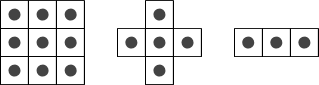
\includegraphics[width=0.6\textwidth]{imagens/elemento_estruturante.png}
\sourceAuthor
\label{fig:elementro_estruturante}
\end{figure}

% ---
\subsection{Erosão}
O processo de erosão é responsável por afinar ou diminuir objetos de uma imagem. Pode ser utilizada para remover componentes de uma imagem que não se tem interesse. A erosão pode ser definida como uma operação de filtragem, em que os elementos da imagem menores que o elemento estruturante são removidos \cite{gonzalesWoods:2008}.

De acordo com \citet{pedriniSchwartz:2008}, a fórmula que representa a operação de erosão em imagens em tons de cinza é definida por:

\begin{figure}[ht]
\centering
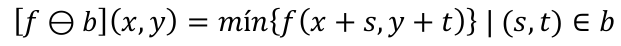
\includegraphics[width=0.6\textwidth]{imagens/erosao_formula.png}
\end{figure}

Onde f representa a imagem de origem e (s, t) pertencem ao elemento estruturante b. Este elemento estruturante é aplicado na imagem e a cada ciclo, o pixel analisado é substituído pelo pixel resultante de menor valor.

A implementação em java para o algoritmo pode ser acessado através do link: \url{https://bit.ly/2rrIuIO}

% ---
\subsection{Dilatação}

A dilatação é um processo que, ao contrário da erosão, aumenta os objetos em uma imagem binária. Um exemplo de utilização pode ser a união de lacunas de uma imagem, onde após a aplicação de uma dilatação, a distância entre estas lacunas diminui ou deixa de existir \cite{gonzalesWoods:2008}. 

De acordo com \citet{pedriniSchwartz:2008}, a fórmula que representa a operação de dilatação em imagens em tons de cinza é definida por:

\begin{figure}[ht]
\centering
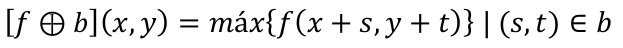
\includegraphics[width=0.6\textwidth]{imagens/dilatacao_formula.png}
\end{figure}

Onde \(f\) representa a imagem de origem e \((s, t)\) pertencem ao elemento estruturante \(b\). Este elemento estruturante é aplicado na imagem e a cada ciclo, o pixel analisado é substituído pelo pixel resultante de maior valor.

É importante ressaltar que as operações de dilatação e erosão são contrárias, mas uma não desfaz a outra. Uma operação de erosão, nem sempre, desfaz corretamente outra operação de dilatação, o mesmo ocorre de maneira inversa.

A implementação em java para o algoritmo pode ser acessado através do link: \url{https://bit.ly/2HYh7ku}

% ---
\subsection{Abertura}

A abertura é geralmente utilizada para suavizar os contornos de um objeto, eliminando, desta forma, as saliências finas. Na operação de abertura as imagens que são menores que os elementos estruturantes são removidas da imagem \cite{gonzalesWoods:2008}.

Segundo \citet{pedriniSchwartz:2008}, o processo de abertura consiste na aplicação de uma erosão, seguida de uma dilatação na mesma imagem, utilizando o mesmo elemento estruturante.

A implementação em java para o algoritmo pode ser acessado através do link: \url{https://bit.ly/2FUz0Lc}

% ---
\subsection{Fechamento}

A operação de fechamento também realiza a suavização da imagem, mas ao contrário da abertura, o fechamento elimina os pequenos buracos e preenche as colunas de um contorno. Sendo assim, separações e áreas menores que o elemento estruturante são completadas \cite{gonzalesWoods:2008}.

Segundo \citet{pedriniSchwartz:2008}, o processo de fechamento consiste na aplicação de uma dilatação, seguida de uma erosão na mesma imagem, utilizando o mesmo elemento estruturante.

A implementação em java para o algoritmo pode ser acessado através do link: \url{https://bit.ly/2jFS47r}

\begin{figure}[ht]
\centering
\caption{\textbf{Aplicações de operações de morfologia matemática em um imagem}}
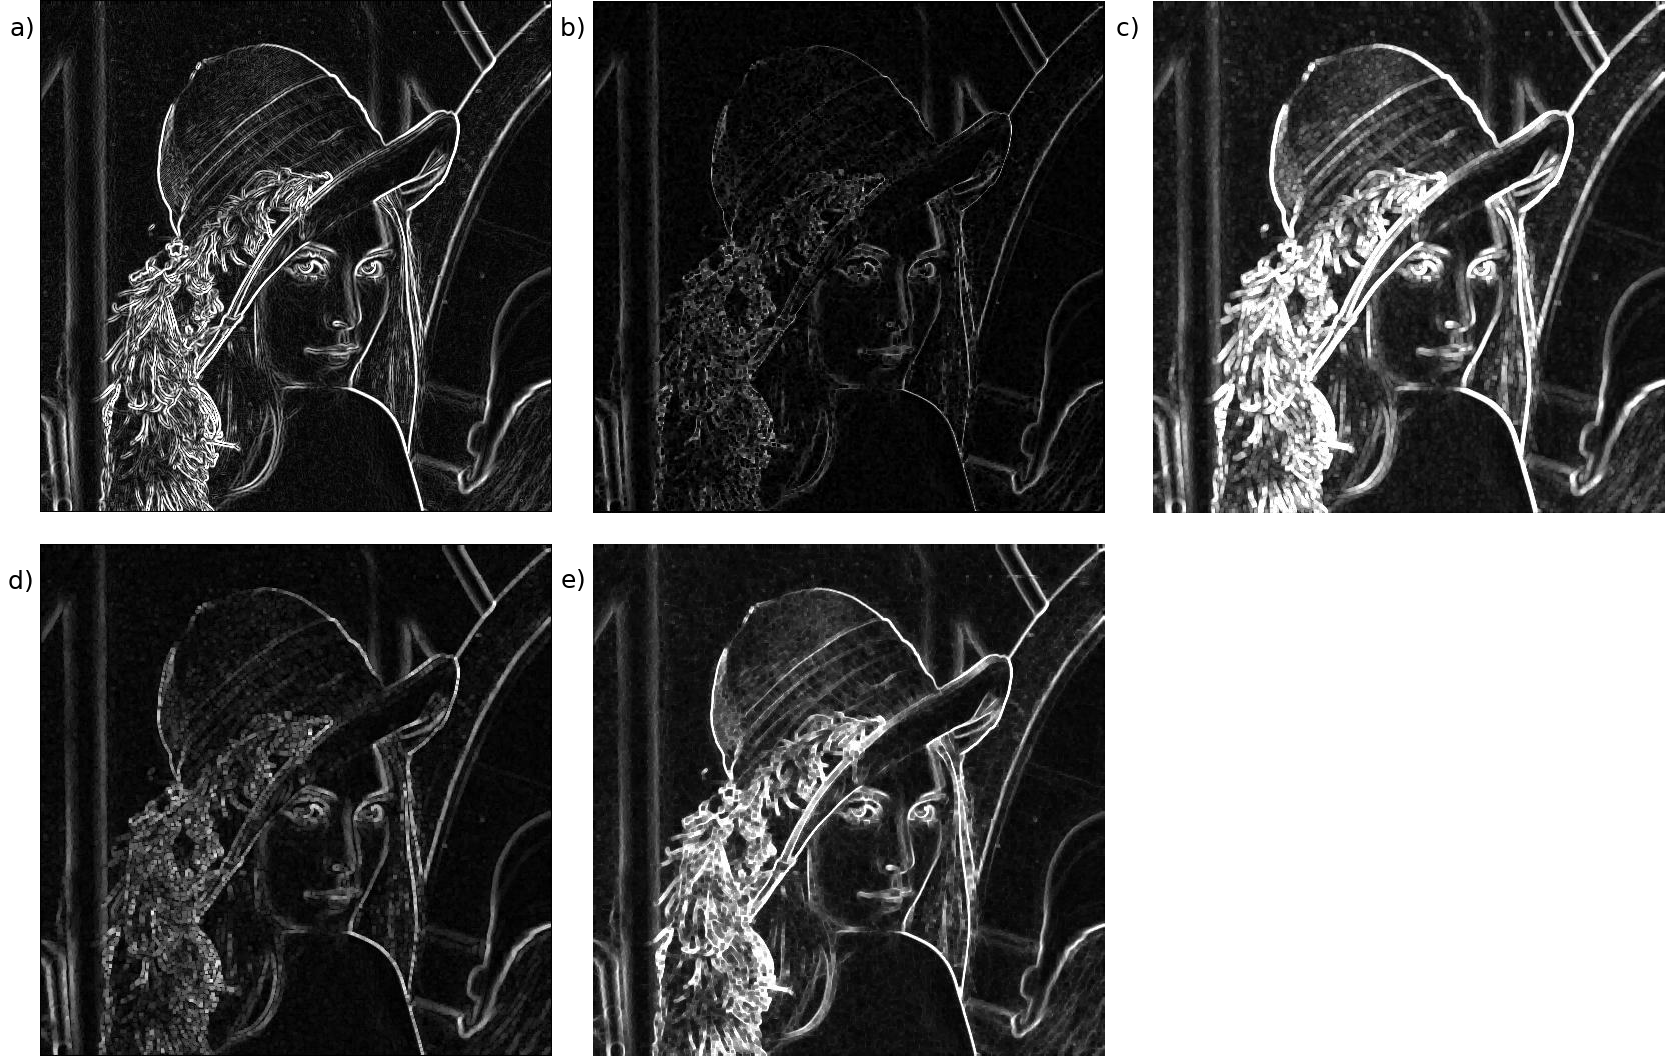
\includegraphics[width=0.9\textwidth]{imagens/morfologia.png}
\sourceAuthor
\label{fig:morfologia}
\end{figure}

Na imagem \ref{fig:morfologia} é apresentada a aplicação de operações de morfologia matemática. A primeira operação apresentada é a erosão (b), seguida da operação de dilatação (c), abertura (d) e fechamento (e).
    
% ---
\section{Afinamento de bordas}    

Os algoritmos de afinamento de bordas tem como objetivo a remoção de pixels redundantes das imagens, produzindo, desta forma, uma simplificação dos objetos da imagem. O principal problema que estes algoritmos enfrentam é determinar com exatidão quais são os pixels redundantes da imagem \cite{guilherme:2007}.

Uma das características mais importantes em um processo de afinamento de bordas é a conectividade. O número de conectividade pode ser definido como sendo o número de transições de branco para preto dentro de uma área ao redor do pixel central \cite{guilherme:2007}.
    
% ---
\subsection{Stentiford}    

O algoritmo de Stentiford adota uma abordagem baseada na utilização de máscaras para o afinamento de objetos. São utilizadas quatro máscaras que são aplicadas de forma sucessiva e ordenada \cite{guilherme:2007}.

\begin{figure}[ht]
\centering
\caption{\textbf{Representa máscaras utilizadas pelo algoritmo de Stentiford}}
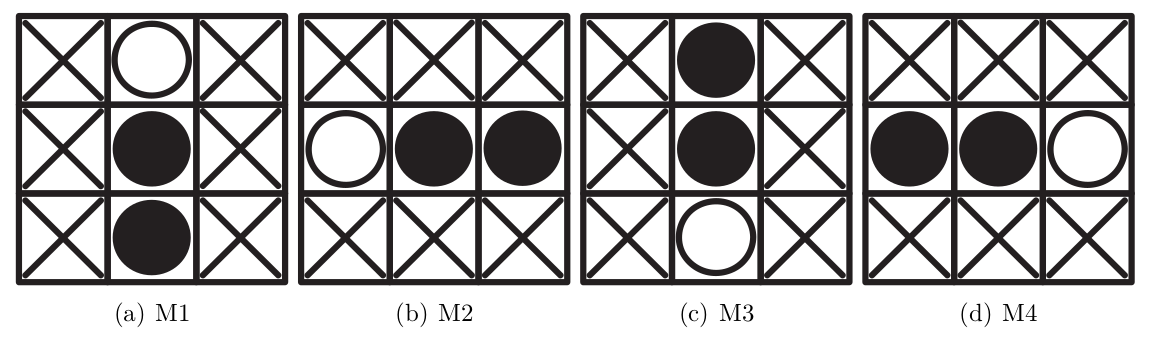
\includegraphics[width=0.7\textwidth]{imagens/stentiford.png}

Fonte: Guilherme (2007, p. 13)
\label{fig:stentiford}
\end{figure}

Na Figura \ref{fig:stentiford} são demonstradas as máscaras utilizadas pelo algoritmo, os círculos brancos representam pixels de valor zero, os círculos pretos representam os pixels de valor 1 e os \(X\) representam os pixels com valores irrelevantes.

Segundo \citet{guilherme:2007}, o algoritmo de Stentiford é composto por seis passos:

\begin{itemize}
\item Percorrer a imagem até encontrar um pixel que se encaixe na máscara M1;
\item Marca o ponto como apagado caso o pixel não seja um ponto final e sua conectividade seja igual a 1;
\item Repetir os passos 1 e 2 para todos os pixels da imagem que se encaixem na máscara M1;
\item Repetir os passos 1, 2 e 3 para as máscaras M2, M3 e M4;
\item Apagar todos os pixels que estejam marcados para serem apagado;
\item Se algum ponto foi apagado no passo 5, os passos a partir do passo 1 devem ser repetidos.
\end{itemize}

A implementação em java para o algoritmo pode ser acessado através do link: \url{https://bit.ly/2I0u0qf}

% ---
\subsection{Zhang Suen}

O algoritmo de Zhang Suen (ZHANG; SUEN, 1984) tem como base a comparação do pixel em processamento com seus 8 vizinhos. A exclusão de pixel por parte do algoritmo somente é realizada mediante a quatro regras. Estas regras têm como objetivo obter a exclusão segura dos pixels, garantindo, desta forma, que áreas interligadas não percam a conectividade e que a eliminação ocorrerá nas bordas do objeto \cite{guilherme:2007}.

\begin{figure}[ht]
\centering
\caption{\textbf{Representa máscaras utilizadas pelo algoritmo de Zhang Suen}}
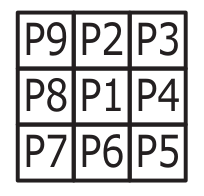
\includegraphics[width=0.3\textwidth]{imagens/zhangsuen_mascara.png}

Fonte: Guilherme (2007, p. 15)
\label{fig:zhangsuen_mascara}
\end{figure}

O algoritmo é composto por duas iterações que fazem uso das quatro regras descritas na sequência. Na primeira iteração, para as regras C e D, serão utilizada as máscaras descritas pela \ref{fig:zhangsuen1} e Figura \ref{fig:zhangsuen2}, respectivamente, na segunda etapa, serão utilizadas as máscaras descritas pela Figura \ref{fig:zhangsuen3} e Figura \ref{fig:zhangsuen4}, respectivamente.

Segundo \citet{guilherme:2007}, para que um pixel seja marcado para exclusão ele deve:

\begin{itemize}
\item Possuir sua conectividade maior que 1;
\item O objeto deve ser composto de pelo menos dois e no máximo seis pixels pretos;
\item Ao menos um dos pixels da primeira máscara deve ser branco;
\item Ao menos um dos pixels da segunda máscara deve ser branco;
\end{itemize}


\begin{figure}[ht]
\centering
\caption{\textbf{pixels P2 ou P8 ou P4 devem ser um pixel branco}}
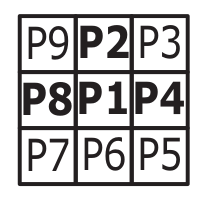
\includegraphics[width=0.3\textwidth]{imagens/zhangsuen1.png}

Fonte: Guilherme (2007, p. 16)
\label{fig:zhangsuen1}
\end{figure}


\begin{figure}[ht]
\centering
\caption{\textbf{pixels P2 ou P8 ou P4 devem ser um pixel branco}}
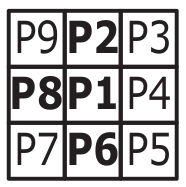
\includegraphics[width=0.3\textwidth]{imagens/zhangsuen2.png}

Fonte: Guilherme (2007, p. 16)
\label{fig:zhangsuen2}
\end{figure}

\begin{figure}[ht]
\centering
\caption{\textbf{pixels P2 ou P4 ou P6 devem ser um pixel branco}}
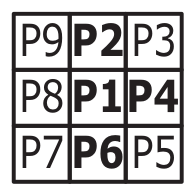
\includegraphics[width=0.3\textwidth]{imagens/zhangsuen3.png}

Fonte: Guilherme (2007, p. 16)
\label{fig:zhangsuen3}
\end{figure}

\begin{figure}[ht]
\centering
\caption{\textbf{pixels P8 ou P6 ou P4 devem ser um pixel branco}}
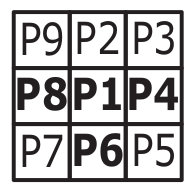
\includegraphics[width=0.3\textwidth]{imagens/zhangsuen4.png}

Fonte: Guilherme (2007, p. 16)
\label{fig:zhangsuen4}
\end{figure}

A implementação em java para o algoritmo pode ser acessado através do link: \url{https://bit.ly/2rrBU5L}

% ---
\subsection{Holt}    

O algoritmo de \citet{holt1987improved} utiliza uma vizinhança 3 x 3 para a análise dos pixels a serem removidos. O formato da matriz permite que seja feita uma análise do pixel central C e seus vizinhos NO, N, NE, O, L, SO, S e SE.

\begin{figure}[ht]
\centering
\caption{\textbf{pixels P8 ou P6 ou P4 devem ser um pixel branco}}
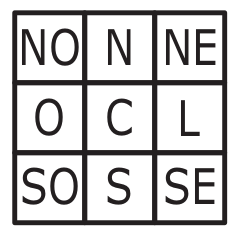
\includegraphics[width=0.3\textwidth]{imagens/holt.png}

Fonte: Guilherme (2007, p. 21)
\label{fig:holt}
\end{figure}

O algoritmo possui duas funções que são definidas por:

\begin{itemize}
\item \(v()\): Retorna verdadeiro se o valor do ponto for o mesmo valor do objeto (valor preto) e falso se o valor do ponto for igual ao valor do plano de fundo (valor branco)
\item \(edge()\): Retorna verdadeiro se o valor processado estiver na borda do objeto e falso se não estiver
\subitem Um pixel está na borda quando sua conectividade é igual a 1 e quando possuir de 2 a 6 vizinhos conectados. 
\end{itemize}

Segundo \citet{guilherme:2007}, o algoritmo de Holt é composto por duas expressões lógicas, onde uma é aplicada na primeira iteração do algoritmo e a outra na segunda iteração. Para um ponto ser removido, o resultado das expressões lógicas devem ser verdadeiros.

Primeira iteração: 
\begin{figure}[ht]
\centering
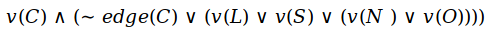
\includegraphics[width=0.8\textwidth]{imagens/holt_formula1.png}
\end{figure}

Segunda iteração:
\begin{figure}[ht]
\centering
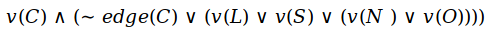
\includegraphics[width=0.8\textwidth]{imagens/holt_formula1.png}
\end{figure}

A implementação em java para o algoritmo pode ser acessado através do link: \url{https://bit.ly/2rr6e0i} 

\begin{figure}[ht]
\centering
\caption{\textbf{Aplicação de algoritmos de afinamento}}

\includegraphics[width=1\textwidth]{imagens/esqueletizacao.png}
\sourceAuthor
\label{fig:esqueletizacao}
\end{figure}

Na Figura \ref{fig:esqueletizacao} são apresentados as aplicações de algoritmos de afinamento. A primeira imagem representa a imagem original (a), seguida do afinamento de Zhang Suen (b), Stentiford (c) e Holt (d). 
   
% ---
\section{Segmentação}  

Segmentação é um processo que consiste em dividir a imagem em regiões. O objetivo deste processo é fazer com que os objetos e áreas de interesse de uma imagem tenham seus pixels agrupados e destacados do restante da imagem. A segmentação é um tema de extrema importância na área de análise de imagens, pois a identificação de partes de imagens que representam elementos de interesse é fundamental \cite{conciAzevedoLeta:2008}.  

A segmentação de imagens é convencionalmente baseada em propriedades dos níveis de cinza de imagens, a descontinuidade e a similaridade. Os métodos da descontinuidade visam a identificação de objetos a partir de mudanças abruptas dos níveis de cinza da imagem, que caracterizam a borda de um objeto. Estes métodos foram tratados do seção XXX. Os métodos de similaridade tem como objetivo agrupar pontos semelhantes da imagem para um determinado conjunto de características \cite{pedriniSchwartz:2008}. Este métodos serão tratados nesta seção.
    
% ---
\subsection{Segmentação baseada em regiões}     

Segmentações baseadas em regiões são métodos que detectam diretamente regiões na imagem, ao invés de detectar bordas que delimitam regiões. Estes algoritmos agrupam pontos que possuem propriedades similares, formando, desta forma, regiões. Um dos principais métodos de segmentação baseada em regiões é o método de crescimento de regiões \cite{pedriniSchwartz:2008}.

O método de crescimento de regiões é um processo de segmentação que tem como início um pixel ou um conjuntos de pixels, que são denominados sementes. Para cada semente, os pixels vizinhos são analisados, caso possuam um nível de similaridade, os pixels são definidos como pertencentes a região da semente. As regiões devem possuir características em comum, considerando algum fator de tolerância. Além disso, regiões devem estar fechadas, possuindo bordas bem delimitadas, de forma que seu interior esteja separado de outros segmentos. \cite{conciAzevedoLeta:2008}.

De acordo com \citet{conciAzevedoLeta:2008}, alguns fatores devem ser considerados na execução do processo de crescimento de regiões. Inicialmente, é necessário que a escolha de semente seja realizada de maneira adequada, representando corretamente a região de interesse, sendo que a semente é o ponto de partida para a execução do método. A definição de critérios de parada do método é outro fator de extrema importância, pois o crescimento deve parar quando não houver mais pixels vizinhos que satisfaçam estes critérios. Estes critérios podem estar relacionados a comparação dos pixels vizinhos, a forma e ao tamanho.

Após a detecção da regiões, comumente é realizada a identificação destas regiões (\textit{label}). Esta identificação consiste em definir um identificador para cada região encontrada na imagem. 

\begin{figure}[ht]
\centering
\caption{\textbf{Exemplo de crescimento de regiões}}
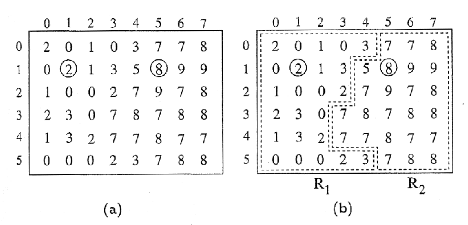
\includegraphics[width=0.8\textwidth]{imagens/crescimento_regiao.png}
\source{\citet{pedriniSchwartz:2008}}
\label{fig:crescimento_regiao}
\end{figure}

Na Figura \ref{fig:crescimento_regiao} é apresentado um exemplo de uma aplicação de crescimento de regiões. (a) representa a imagem origem. (b) representa uma segmentação utilizando como limiar (T) 4, desta forma, a diferença absoluta entre a semente e o valor do pixel analisado deve ser menor do que 4 para que o pixel seja considerado pertencente a região da semente. Os pontos (1, 1) e (1,5) representam as sementes utilizadas para o método. O predicado P, utilizado para adicionar um pixel em uma região, pode ser observado na fórmula:

\begin{figure}[ht]
\centering
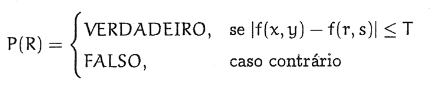
\includegraphics[width=0.5\textwidth]{imagens/crescimentoregiao_formula.png}
\end{figure}

Onde \(f(r,s)\) representa a semente e \(f(x, y)\) representam os pixels conectados a semente.
    
% ---
\subsection{Método de Contornos Ativos}     

Os métodos de contornos ativos, também conhecidos como Snakes, são técnicas que tem como objetivo a extração das bordas de objetos da imagem. Estas técnicas são caracterizadas para uma curva, que é ajustada de acordo com o contorno do objeto. A técnica é iniciada a partir de um contorno arbitrário que é evoluído até a correta identificação do objeto de interesse \cite{conciAzevedoLeta:2008}.

O ajuste da curva é realizado levando em consideração forças internas e externas à curva. O objetivo da energia interna é manter a continuidade e suavidade do contorno, levando em consideração o formato do objeto. Já a energia externa é responsável por buscar valores onde há maior variável entre o pixel e seus vizinhos, o que caracteriza uma borda \cite{kass:1988}.

\begin{figure}[ht]
\centering
\caption{\textbf{Exemplo na execução do método Snakes}}
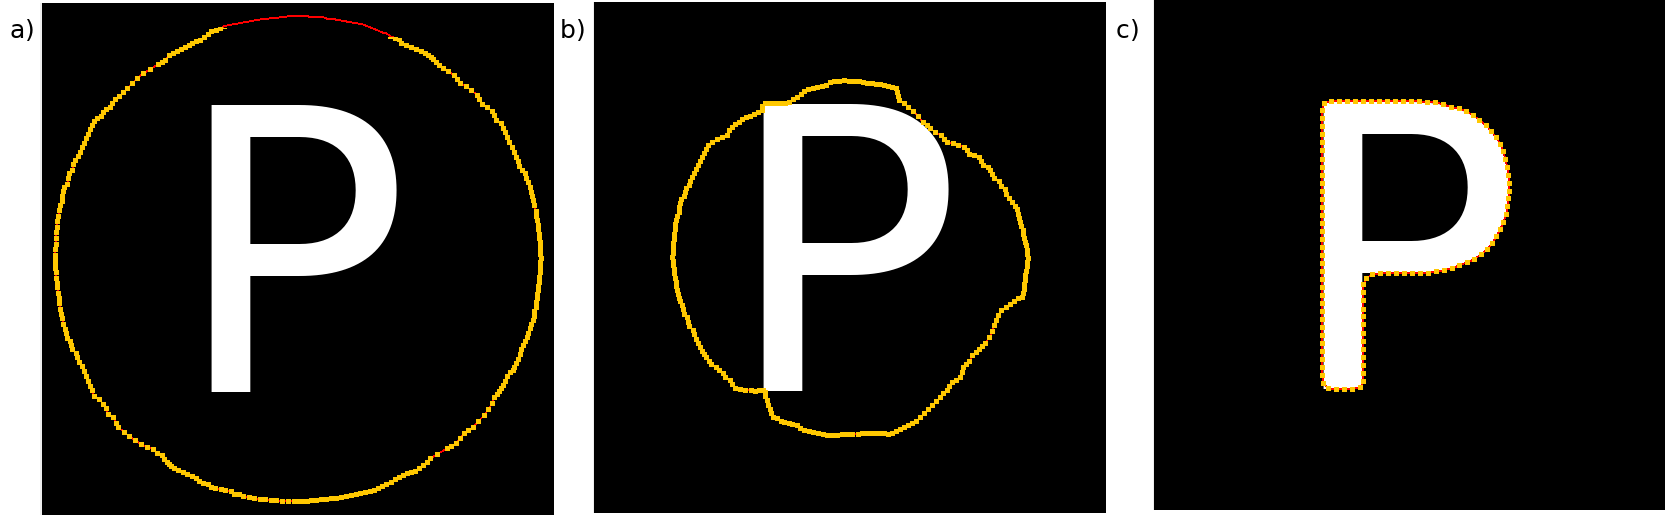
\includegraphics[width=1\textwidth]{imagens/snake.png}
\sourceAuthor
\label{fig:snake}
\end{figure}

\citet{de2013classroom}

Na Figura \ref{fig:snake} é demonstrado uma execução do método de Snakes. (a) é o contorno inicial. (b) é o contorno resultante após aplicação de algumas etapas. (c) contorno final.

A implementação em java para o algoritmo pode ser acessado através do link: \url{https://bit.ly/2jG3YxY}

\section{Considerações}

Neste capítulo foi apresentado o referencial teórico referente a PDI, cumprindo, desta forma, o primeiro objetivo específico do trabalho. Foram abordadas as principais técnicas de PDI relacionadas a transformações geométricas, filtros passa-baixa, filtros passa-alta, morfologia matemática, afinamento de bordas e técnicas de segmentação. Todas as técnicas apresentadas estão implementadas na ferramenta VISNode que será aborda na sessão \ref{sec:visnode}.

No próximo capítulo serão abordados conceitos referente a gamificação. São abordados temas referente a sua diferença em relação a simulação e jogo, sua aplicação na educação e elementos da gamificação.

% ----------------------------------------------------------
% Gamificação
% ----------------------------------------------------------
\chapter{Gamificação}

A gamificação é um tópico bastante discutido nos últimos anos, estando presente no meio empresarial, acadêmico e nas mais diversas áreas de conhecimento. A gamificação é encarada como uma ferramenta de auxílio para o estímulo e o engajamento de pessoas no desenvolvimento de atividades, fazendo uso de elementos de jogos e suas características \cite{quadros2016gamificaccao}.

A gamificação tem sido aplicada com o objetivo de melhorar a experiência e engajamento de usuários \cite{quadros2016gamificaccao}. Segundo \citet{deterding2011game}, a gamificação é um conceito que pode ser aplicado nos mais diversos campos de pesquisa, estando presente em áreas de ciências humanas, computação, finanças, saúde e educação. É um termo que deve ser utilizado para sistemas que utilizam elementos de jogos, e não para cenários que utilizam games. 

Levando em consideração este cenário propício, a gamificação se apresenta como uma ferramenta com grande potencialidade de aplicação. Isso se faz possível devido a linguagem e metodologia dos games serem bastante populares, sendo aceitos naturalmente pelas gerações que cresceram interagindo com esse tipo de entretenimento \cite{fardo2013gamificaccao}. Segundo \citet{deterding2011game}, a gamificação é um fenômeno emergente, que se aproveita da popularidade dos jogos digitais e de suas capacidades de motivar ações, resolver problemas e potencializar aprendizagens em diversas áreas do conhecimento

Um dos autores precursores na teorização da gamificação foi \citet{mcgonigal2011reality}, afirmando que promover o engajamentos das pessoas em atividades do cotidiano, fazendo uso da lógica de jogos na vida real, pode auxiliar no desenvolvimento de um mundo melhor.

Dentre as principais características da gamificação estão a utilização de elementos de jogos digitais, tais como: narrativa, sistema de \textit{feedback}, sistema de recompensas, gerenciamento de conflito, cooperação, competição dirigida, objetivos e regras claras, níveis, tentativa e erro, diversão, interação, interatividade, etc. Estas características são importantes para obter o envolvimento do sujeito, o que pode ser encontrado na relação entre jogadores e jogos \cite{deterding2011game}.

Este capítulo trata de conceitos referente a gamificação. É abordada sua diferença em relação a simulação e jogo, sua aplicação na educação e elementos da gamificação.

% ---
\section{Jogo, Simulação, Gamificação}

Jogo, simulação e gamificação são conceitos que muitas vezes são confundidos. Esta confusão acontece por estes conceitos compartilharem características comuns.

Definir o que é um jogo não é uma tarefa fácil devido a grande quantidade e diversidade de jogos existente. Há, por exemplo, jogos de tabuleiro, como xadrez e damas, também há jogos digitais, como jogos de console e computador e também há jogos esportivos como Futebol, Rugby, entre outros. Desta forma, o fato de um produto ser eletrônico não o define como sendo um jogo. Um jogo normalmente é caracterizado pela existência de um objetivo, além de regras específicas. Sendo assim, um jogo pode ser definido como sendo um sistema onde jogadores estão engajados em um desafio que é definido por regras, interatividade e \textit{feedback} \cite{kaap:2014}. 

Dentro da área de jogos existe uma categoria denominada \textit{Serious Game}, que são jogos desenvolvidos com o objetivo de resolver problemas reais. A gamificação e os \textit{serious game} estão relacionadas, pois ambos fazem uso de conceitos de jogos para conquistar algo a mais. Um \textit{Serious Game} é um jogo real, enquanto a gamificação faz uso de uma série de ferramentas relacionadas a jogos, como, por exemplo a mecânica ou dinâmica de jogo, design do jogo, psicologia dos jogos, entre outros \cite{dorling2012software}

A simulação também está relacionada com a ideia de jogo. Mas diferente de um jogo, a simulação é um ambiente onde usuários podem praticar ações e comportamentos do mundo real em um mundo virtual. Um simulador de voo é um exemplo, a partir dele é possível que um piloto simule diversas manobras como a decolagem e a aterrissagem de uma aeronave.

\begin{figure}[ht]
\centering
\caption{\textbf{Contextualização da gamificação }}
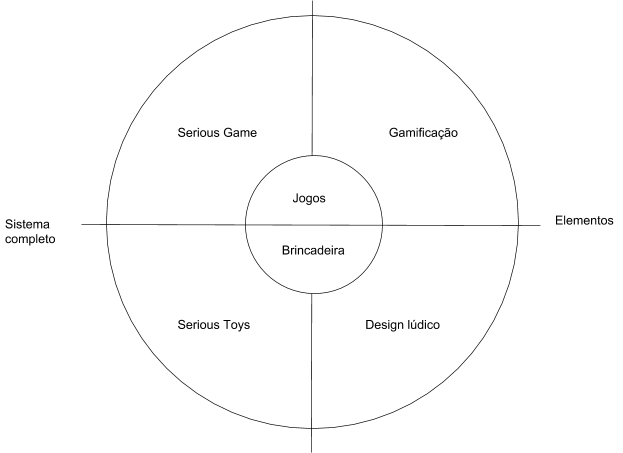
\includegraphics[width=0.9\textwidth]{imagens/gamificacao.png}
\source{Adaptado de \citet{deterding2014gameful}}
\label{fig:gamificacao}
\end{figure}

A Figura \ref{fig:gamificacao} contextualiza a gamificação, fazendo uma divisão em 4 sessões. As sessões acima do eixo horizontal compõem abordagens que fazem uso de conceitos de jogos (mais formal), já as sessões abaixo do eixo horizontal compõem abordagens que fazem uso de brincadeiras (livre e descontraída). Também há outra divisão realizada no eixo vertical da imagem, onde é separado abordagens que fazem uso de jogos  de abordagens que somente utilizam elementos de jogos.

A gamificação é uma abordagem que visa facilitar a aprendizagem e incrementar a motivação, através da utilização de conceitos provenientes dos jogos, como superar desafios, receber recompensas e ganhar pontuação. Um dos objetivos da gamificação é atrair a atenção da pessoa e motivá-la a executar a tarefa proposta, criando um ambiente onde haja um maior envolvimento \cite{kaap:2014}. Semelhante ao que acontece com o uso de \textit{serious game}, a gamificação utiliza jogos para um propósito diferente do uso normal para o entretenimento \cite{deterding2011game}.

% ---
\section{Gamificação na educação}

O sistema de educação formal apresenta uma área bastante fértil para a aplicação da gamificação, pois é uma área que apresenta diversas falhas em engajar estudantes que estão cada vez mais inseridos no contexto tecnológico e das mídias sociais. Além disso, estes indivíduos já possuem grande interação com jogos, o que facilitaria na aplicação desta metodologia. Outro fator é o de que os estudantes se mostram mais desinteressados pelos métodos passivos de ensino, onde os educadores transmitem o conhecimento \cite{fardo2013gamificaccao}. 

Uma das grandes vantagens de utilizar a gamificação para estudantes é de proporcionar um sistema onde eles consigam visualizar o efeito de suas ações e aprendizagens na medida que vão aprendendo. Desta forma, os indivíduos sentem que estão contribuindo para algo maior e de maior importância. Estes objetivos podem ser alcançados através da aplicação de elementos de jogos, se aplicados cuidadosamente \cite{fardo2013gamificaccao}. Conforme \citet{kaap:2014}, a gamificação pode ser utilizada com a finalidade de encorajar o aprendizado através de todos os elementos de jogos digitais que se demonstrarem apropriados para tal finalidade.  

Segundo \citet{fardo2013gamificaccao}, um dos grandes desafios da utilização da gamificação para o ensino é aplicá-la corretamente. Uma prática pedagógica pouco eficaz é focar somente em um mecanismo de pontuação e recompensas, visando apenas a obtenção de resultados finais, e não levando em consideração a construção da aprendizagem e a experiência obtida por parte dos estudantes. O autor salienta que o importante é buscar práticas pedagógicas que não se limitem a motivar os estudantes na busca por recompensas, sem levar em consideração os processos de reflexão, colaboração e de cooperação.

Segundo \citet{fardo2013gamificaccao}, a utilização da gamificação como uma ferramenta pedagógica não deve ser encarada como a solução de todos os problemas da educação. Sua utilização requer compreensão por parte dos educadores, sendo que estes são responsáveis por sua aplicação e devem identificar se sua utilização está realmente potencializando a aprendizagem e a participação dos estudantes. Para o autor, a gamificação pode ser vista como um caminho na busca por soluções que são necessárias para o atual sistema de educação.

Portanto, a ideia por trás da aplicação da gamificação na educação é adicionar elementos de jogos para envolver os alunos e motivar seu engajamento, permitindo um \textit{feedback} imediato e a oportunidade de fracassar. A abordagem tem com objetivo transformar a aprendizagem passiva em um processo ativo, motivando os alunos a estudar o conteúdo trabalhado.

% ---
\subsection{Motivação intrínseca e extrínseca}

Uma questão bastante polêmica em torno da gamificação é comparação entre motivação intrínseca e motivação extrínseca. É argumentado que a gamificação faz uso de muitos fatores externos (extrínsecos) para motivar os alunos e é deixado de lado os fatores internos (intrínsecos) \cite{fardo2013gamificaccao}.

A motivação intrínseca é aquela originada pelo próprio indivíduo. O envolvimento do indivíduo ocorre por vontade própria,  pois é motivado por interesse, desafio ou prazer. Além da busca por novidades, curiosidade e vontade de aprender algo novo. Desta forma, o indivíduo participa de uma atividade pois ela proporciona satisfação \cite{busarello2016gamificaccao}.

De maneira contrária, a motivação extrínseca é baseada no mundo que envolve o indivíduo de forma externa. Tem como origem o desejo em obter alguma recompensa externa, como, por exemplo, pontos, prêmios e classificações ou evitar uma punição. Desta forma, através da motivação extrínseca, um indivíduo não é motivado por fatores internos, em vez disso, é motivação pela recompensa que será obtida por realizar uma determinada tarefa \cite{busarello2016gamificaccao}.

% ---
\section{Elementos gamificação}

Elementos de jogos aplicados a gamificação como narrativas, metas, regras, \textit{feedbacks} e desafios podem contribuir para uma experiência agradável em um ambiente gamificado, pois favorecem a participação de maneira voluntária por parte do indivíduo \cite{busarello2016gamificaccao}.

Nesta seção serão apresentado os principais elementos utilizados em soluções gamificadas. Como já foi descrito anteriormente, a gamificação faz uso de elementos de jogos, desta forma, os elementos descritos nesta seção são originários de elementos de jogos.

% ---
\subsection{Narrativas}

A narrativa é um elemento fundamental no contextos de games, pois este é o elemento chave para o acontecimento de eventos e para justificar as ações de jogadores. Uma boa história pode contribuir para o envolvimento do jogador através da interatividade proporcionada por ela  \cite{fardo2013gamificaccao}. Sendo \citet{kaap:2014}, a utilização de histórias, como um elemento gamificado, fornece relevância e significado para experiências obtidas pelo usuário, fornecendo um cenário propício para a aplicação de tarefas.

Segundo \citet{fardo2013gamificaccao} é mais agradável aprender novas informações e adquirir novos conhecimento que estejam relacionados a um determinado contexto, e a narrativa pode ser uma fonte para fornecer contextos. Além disso, envolver o aluno em uma história pode contribuir para que a aprendizagem se torne mais poderosa, sendo que uma história focada em ajudar os alunos a resolver problemas, contribui para a educação do aluno e facilita a memorização do conteúdo abordado.

% ---
\subsection{Metas, Regras e Objetivos}

A meta consiste no propósito pelo qual um indivíduo realiza uma determinada tarefa, é aquilo que o indivíduo persegue constantemente. Desta forma, a atividade se apresenta como sendo o desejo pelo qual um indivíduo possui em atuar em uma determinada atividade \cite{bunchball2016gamification}. Segundo \citet{kaap:2014}, metas contribuem para a visualização de propósitos, foco e resultados.

As regras têm como objetivo restringir ações por parte do indivíduo, desta forma, determinado a maneira de como o indivíduo agirá para completar os desafios do ambiente. As regras buscam equilibrar o nível de complexidade com o nível de conhecimento do sujeito, favorecendo, desta forma, a criatividade e o pensamento estratégico \cite{bunchball2016gamification}.

O objetivo é aquilo que o indivíduo deve realizar. Objetivos devem ser apresentados de forma clara, para que não haja confusão e aumento da complexidade devido a ambiguidade do objetivo. Normalmente, um jogo possui mais de um objetivo, que vão sendo organizados ao decorrer da iteração. Quando há objetivos muito complexos, estes podem ser quebrados em objetivos menores, para que o indivíduo consiga atingir o objetivo maior. Esta subdivisão de desafios permite ao indivíduo identificar seu progresso em relação ao objetivos maiores \cite{fardo2013gamificaccao}.

% ---
\subsection{Pontos}

Este elemento pode ser utilizado para diversos propósitos. Uma de suas aplicações é demonstrar o progresso do usuário, servindo como \textit{feedback}, de forma que seja possível identificar se o usuário está agindo de maneira correta. Este elemento também pode servir como estímulo, de forma que o usuário buscará uma maior pontuação \cite{kaap:2014}. 

% ---
\subsection{Medalhas}

Medalhas são a comprovação de que uma determinada tarefa foi realizada com mérito ou excelência. Em um sistema gamificado, o uso de medalhas ocorre através de uma indicação visual de que se tenha alcançado um determinado nível ou se tenha comprido um determinado conjunto de objetivos. Para \citet{deterding2011game}, medalhas são apresentadas em algum lugar ou de alguma forma para que outros jogadores possam observar as conquistas e a realização do jogador. O uso de medalhas pode motivar um maior envolvimento por parte dos usuários do sistema, devido a busca por um determinado emblema.
    
% ---
\subsection{Recompensas e Conquistas}    

Recompensas apresentadas após a finalização de ações podem estimular o comportamento e o envolvimento da pessoa em um sistema gamificado. Na gamificação, o mecanismo de recompensas ocorre através do ganho de pontos ou algo equivalente \cite{kaap:2014}. Os seres humanos são motivados pelo recebimento de recompensas, seja pela satisfação pessoal ou através de medalhas ou presentes \cite{quadros2016gamificaccao}.

A conquista é um importante elemento para a motivação, sendo que através da resolução de tarefas de alta dificuldade é possível obter a gratificação e reconhecimento da realização conquistada \cite{quadros2016gamificaccao}. Para \citet{busarello2016gamificaccao}, recompensar é uma forma de medir o desempenho do jogador utilizando pontuação e formas de prêmios, após a finalização de tarefas ou níveis no jogo.

Recompensas podem ser adquiridas após a conclusão de uma tarefa ou através da medição de desempenho do aluno ao completar uma tarefa. De acordo com \citet{quadros2016gamificaccao}, a utilização de recompensas através de uma medição pode aumentar a motivação intrínseca, pois o aluno terá um \textit{feedback} de quão bem ele está. Se as recompensas forem aplicadas corretamente, podem ter um grande efeito motivacional aos alunos.
    
% ---
\subsection{Níveis e \textit{rankings}}        

Os níveis são caracterizados por diferentes categorias que envolvem graus de habilidade e conhecimento. Um nível demonstra um grau de realização, comprovando um determinado nível de conhecimento \cite{kaap:2014}. Segundo \citet{quadros2016gamificaccao}, níveis podem ser definidos como sendo um sistema pelo qual ocorre a recompensa através do acúmulo de pontos.

O uso de níveis é um dos maiores componentes para a ocorrência de motivação. Pessoas conseguem determinar seus esforços para a realização de um determinado desafio e através disso se motivar e se esforçar cada vez mais. Podem ser utilizados para identificar o nível de habilidade e conhecimento do indivíduo no sistema.

A utilização de \textit{rankings} permite aos jogadores uma forma de interagir socialmente em torno do jogos, podendo comparar seu progresso com outros jogadores. Também fornece uma forma para que os jogadores possam se vangloriar quando alcançarem resultados melhores. É importante que este \textit{ranking} esteja inserido dentro do contexto do problema, de forma que ele possa competir com os demais usuários \cite{quadros2016gamificaccao}.
    
% ---
\subsection{\textit{Feedback}}            

O \textit{feedback} é um recurso pelo qual jogadores podem visualizar o resultado de suas ações, tornando-se um poderoso elemento para tornar o usuário mais focado e permitir modificar suas estratégias para melhorar seu desempenho. Este elemento, auxilia na construção do conhecimento através da integração entre o indivíduo e o sistema, onde o retorno do sistema pode ao aumentar a experiência do aprendizado \cite{fardo2013gamificaccao}.
    
% ---
\subsection{Desafios}                

Os desafios são impostos aos usuários para direcionar o que deve ser feito dentro do cenário proposto. É importante que o usuário sempre tenha algo interessante para fazer, contribuindo para uma melhor experiência. Além disso, é interessante disponibilizar diversas opções neste ambiente, pois usuários podem possuir perfis diferentes \cite{fardo2013gamificaccao}.

Segundo \citet{busarello2016gamificaccao}, os indivíduos têm interesse em resolver desafios que possuem um nível de dificuldade equilibrado, ou seja, não podem ser nem muito fáceis nem muito difíceis. Este equilíbrio entre os níveis de dificuldade e habilidade podem colaborar para o fluxo da atividade, contribuindo para o motivação.
    
% ---
\subsection{Conflito, Competição e Cooperação}                    

As pessoas atingem um nível mais elevado de satisfação ao comparar seu desempenho com o de outras pessoas. Este ambiente competitivo pode aumentar o desempenho. Elementos de jogos instigam esse tipo de desejo, fazendo uso de \textit{rankings} para exibir os resultados e celebrando os vencedores  \cite{bunchball2016gamification}. Alguns jogos fazem uso de uma lista contendo os 10 mais bem classificados, utilizando a exposição para indicar novos níveis e recompensas alcançadas.

\section{Considerações}

Neste capítulo foi apresentado o referencial teórico referente a gamificação, cumprindo, desta forma, o segundo objetivo específico do trabalho. Foi abordado o conceito de gamificação, sua aplicabilidade como ferramenta educacional e seus principais elementos .

No próximo capítulo serão apresentados trabalhos relacionados ao trabalho desenvolvido. O primeiro trabalho apresentado (sessão \ref{sec:javavis}) é uma ferramenta que foi desenvolvida com o objetivo de auxiliar no ensino e aprendizagem de PDI. O segundo trabalho apresentado (sessão \ref{sec:classrom}) é uma ferramenta que foi desenvolvida visando melhorar o engajamento de estudantes, para isso, ela foi desenvolvida utilizando elementos da gamificação.

% ----------------------------------------------------------
% Trabalhos correlatos
% ----------------------------------------------------------
\chapter{Trabalhos correlatos}

Neste capítulo são apresentados trabalhos relacionados à área de pesquisa deste projeto. O objetivo é identificar e avaliar os propostas que outros autores utilizaram para tratar do tema do presente estudo.

% ---
\section{JavaVis: An Integrated Computer Vision Library for Teaching Computer Vision}
\label{sec:javavis}

A pesquisa de \citet{cazorla2015javavis} propõe o desenvolvimento de um \textit{framework} para estudar visão computacional e tópicos semelhantes. Esta ferramenta foi chamada de JavaVis. Esta ferramenta é dividida em 3 áreas. A primeira área é denominada JavaVis2D, por onde o sistema é iniciado. Esta área está relacionada com a visão computacional tradicional, onde é possível utilizar diversos algoritmos já implementados, e também que os próprios alunos criem novos algoritmos. 

JavaVisDesktop é uma outra área do software, que permite a conexão de uma sequência de algoritmos e a manipulação de seus parâmetros. Esta área foi construída para facilitar a manipulação dos algoritmos por parte do aluno, tendo em vista que a manipulação individual de algoritmos através de área 2D pode ser difícil, devido a grande quantidade de tentativas para ajustar corretamente os parâmetros. Por final, existe a área 3D que tem como objetivo permitir a manipulação de imagens 3D.

O objetivo do JavaVis é prover uma ferramenta que seja fácil de utilizar e aprender conceitos relacionados à visão computacional, sempre tendo em vista que o desenvolvimento de novos algoritmos deve ser uma tarefa fácil. O JavaVis permite a manipulação de algoritmos através de uma interface gráfica, possibilitando alteração de parâmetros de algoritmos visualmente. É uma ferramenta que foi construída objetivando facilitar a aprendizagem de estudantes.

% ---
\subsection{JavaVis2D}

O JavaVis2D é uma área da ferramenta que possui diversos algoritmos de visão computacional implementados. Dentre eles podem ser encontrados funções de manipulação e transformações de cores, como rotação, espelhamento, ruído, conversão para tons de cinza, etc. Também são encontrados algoritmos de convolução, ajuste de imagem como brilho e contraste, segmentação como Binarização e \textit{Kmeans}, manipulação geométrica, detecção de bordas como Canny, Susan e Grad, morfologia matemática como erosão e dilatação e também algoritmos de esqueletização. 

A biblioteca permite a criação de funções por parte do aluno, isso é possível através da implementação de uma classe Java contendo a implementação de uma função, juntamente com seus parâmetros de entrada e saída. Desta forma, segundo os autores, o aluno precisa somente se concentrar no desenvolvimento da função, a biblioteca se encarrega exibir as imagens na interface e aceitar os parâmetros de entrada.

\begin{figure}[ht]
\centering
\caption{\textbf{Aplicação do processo de binarização }}
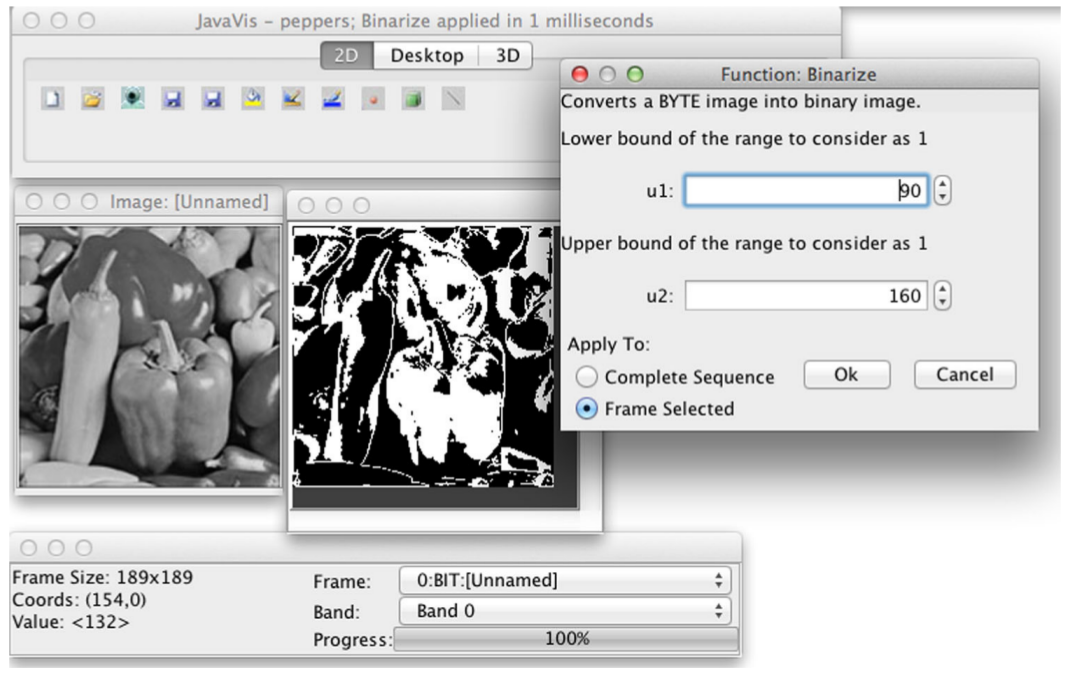
\includegraphics[width=0.8\textwidth]{imagens/javavis_2d.png}
\source{\citet{cazorla2015javavis}}
\label{fig:javavis_2d}
\end{figure}

% ---
\subsection{JavaVisDesktop}

Está área do projeto tem como objetivo proporcionar ao aluno uma melhor maneira para visualizar partes de um processamento de imagem. Portanto, é possível utilizar diferentes algoritmos em ordem para construir outro de maior complexidade. É possível construir uma sequência de funções, semelhante a um autômato. Cada estado na sequência corresponde a um algoritmo da biblioteca JavaVis2D, e este estado apresenta o resultado de execução de seu algoritmo, possibilitando a visualização de cada etapa do processo.

Esta abordagem em etapas permite ao estudante ajustar facilmente os parâmetros de cada algoritmo, sendo possível observar a consequência de cada alteração na sequência completa. Após a conclusão do sequenciamento dos algoritmos e dos ajustes de parâmetros, é possível gerar uma nova função para a biblioteca JavaVis2D. Esta nova função conterá a sequência de funções com seus respectivos parâmetros.

Segundo os autores, JavaVisDesktop é uma ferramenta interessante para identificar os diferentes comportamos de cada algoritmo. Por exemplo, o estudante é capaz de verificar a diferença da aplicação do algoritmo de Canny utilizando diferentes valores para o parâmetro de sigma, possibilitando, desta forma, a escolha o valor mais adequado para o problema enfrentado. Os autores relatam que esta funcionalidade é amplamente apreciada pelos estudantes, pois agiliza a implementação de novos algoritmos.

Na Figura \ref{fig:javavis_desktop} é demonstrada a sequência de três funções, que são: carregamento da imagem, suavização Gaussiana e Canny. Na figura existe uma janela que possibilita a alteração dos parâmetros da função de Canny. Também é possível visualizar o resultado da execução de cada função.

\begin{figure}[ht]
\centering
\caption{\textbf{Ambiente JavaVisDesktop}}
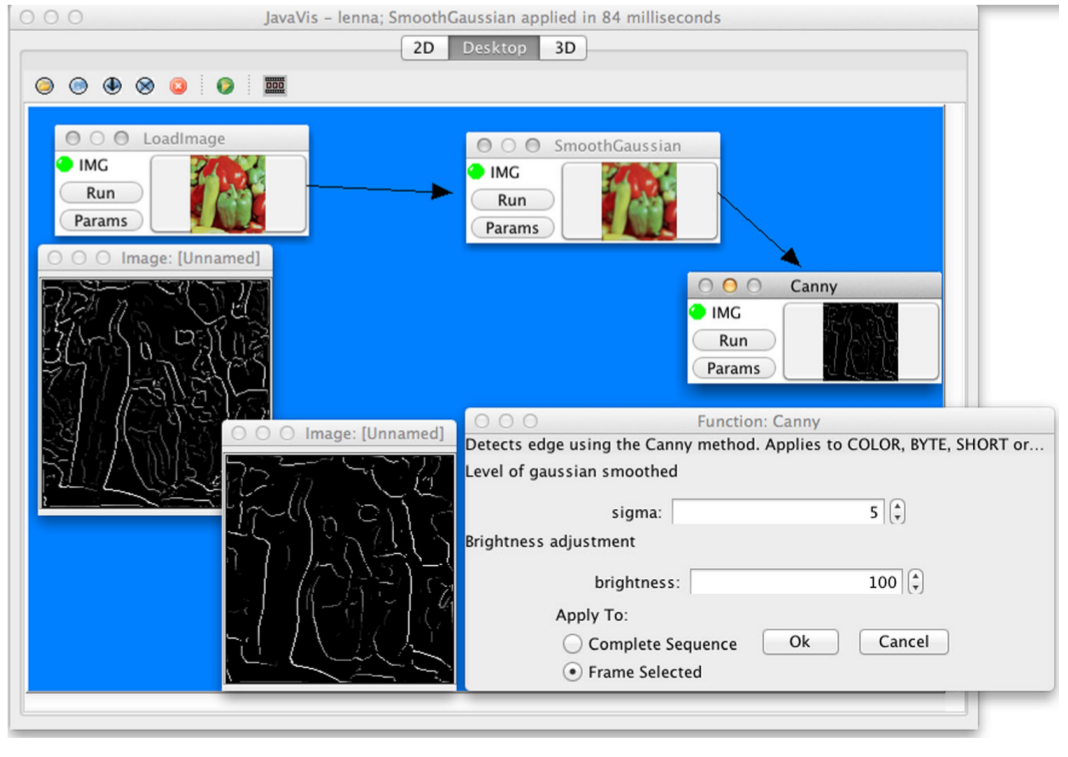
\includegraphics[width=0.8\textwidth]{imagens/javavis_desktop.png}
\source{\citet{cazorla2015javavis}}
\label{fig:javavis_desktop}
\end{figure}

% ---
\subsection{JavaVis3D}

Esta área da ferramenta tem como objetivo permitir a manipulação de imagens 3D. A maior parte de entidades geométricas estão implementadas no core do JavaVis3D. Entidades como pontos, vetores, segmentos e planos estão incluídos neste pacote, sendo possível utilizados para a aplicação de manipulações nas imagens. A interface foi construída utilizando a API 3D do Java, baseada em OpenGL.

A Figura \ref{fig:javavis_3d} demonstra o JavaVis3D \textit{framework}. A janela a direita controla a posição da cena. O usuário pode navegar pela cena utilizando esta janela.

\begin{figure}[ht]
\centering
\caption{\textbf{Ambiente JavaVis3D}}
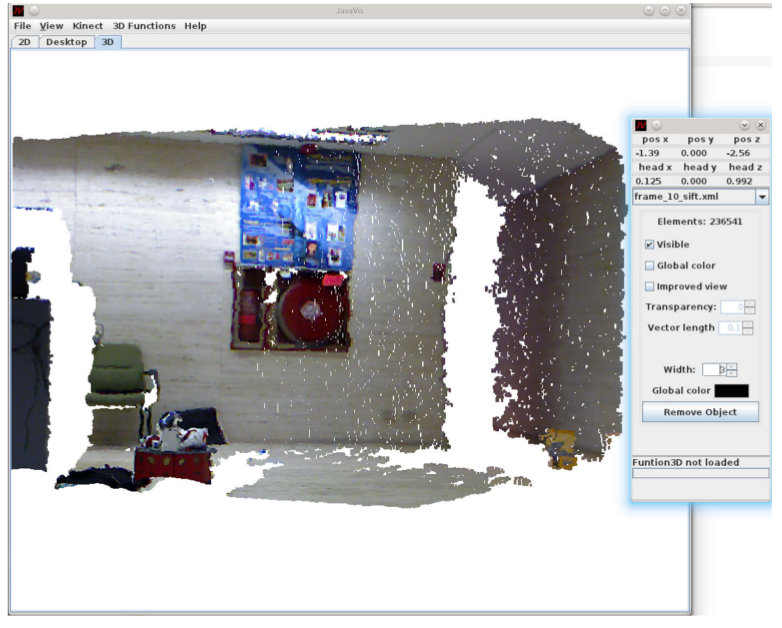
\includegraphics[width=0.8\textwidth]{imagens/javavis_3d.png}
\source{\citet{cazorla2015javavis}}
\label{fig:javavis_3d}
\end{figure}

% ---
\subsection{Resultados obtidos}

Segundo os autores, o JavaVis foi utilizado em diversos cenário relacionados à visão computacional, como inteligência artificial e diversos trabalhos de conclusão da universidade de Alicante (Espanha). Esta ferramenta foi utilizada em dois níveis. O primeiro consiste na utilização dos algoritmos já implementados na biblioteca, possibilitando a observação de seus funcionamentos quando a teoria é apresentada. O segundo nível consiste no desenvolvimento de novos algoritmos pelos alunos.

A ferramenta foi utilizada em sala de aula. Os autores, primeiramente, introduziram a ferramenta para a turma, demonstrando as principais funcionalidades e a aplicação de um exemplo guiado da utilização do JavaVis. Após esta introdução, foi solicitado para os alunos desenvolverem suas próprias funções. Esta abordagem contribuiu para melhorar o entendimento dos algoritmos pelos alunos, sendo que os estudantes puderam identificar o comportamento de diversas funções e tiveram a oportunidade de desenvolver suas próprias funções.

Os autores aplicaram diversas tarefas ao longo de 10 anos. Um exemplo pode ser observado na Figura \ref{fig:javavis_avaliacao}, onde os alunos tiveram que construir uma função capaz de identificar a quantidade de moedas existentes na imagem. Primeiramente, os estudantes utilizaram a área de Desktop para identificar os melhores métodos e seus respectivos parâmetros. Posteriormente, os alunos criaram uma nova função no JavaVis capaz de executar a tarefa proposta.

Para os autores, o JavaVis possui algumas funcionalidades que permitem ao estudante uma maneira simples de aprender visão computacional. Uma delas é a simplicidade de implementação de novos métodos. Outra é a possibilidade do estudante visualizar cada etapa do processamento de algoritmos, devido a sequenciamento de técnicas para a composição de um algoritmo de maior complexidade.

\begin{figure}[ht]
\centering
\caption{\textbf{Exemplos de tarefa aplicada aos estudantes}}
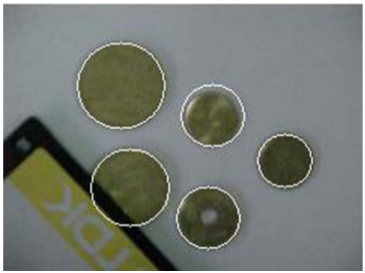
\includegraphics[width=0.7\textwidth]{imagens/javavis_avaliacao.png}
\source{\citet{cazorla2015javavis}}
\label{fig:javavis_avaliacao}
\end{figure}

% ---
\section{Classroom Live: a software-assisted gamification tool}
\label{sec:classrom}

A pesquisa de \citet{de2013classroom} tem por objetivo conseguir engajar os estudantes da US Air Force Academy. Para isso, foi desenvolvido um sistema cliente/servidor para servir como aporte para aulas gamificadas. O sistema é chamado de Classroom Live, e este faz uso do de computadores e acesso wireless para prover uma experiência \textit{online} e interativa de aprendizagem. Ao acessar o software, o aluno recebe “\textit{quests}” que são preparadas pelo instrutor. O instrutor pode acessar uma aplicação diferente para analisar a performance do estudante e recompensas em tempo real.

Os autores desenvolveram o software visando a utilização em aulas do curso de ciência da computação, e que pudesse utilizar a infraestrutura já existente, como computadores e acesso a internet. O desenvolvimento da aplicação foi influenciado pelo \textit{feedback} de alunos e instrutores, servindo como guia para o desenvolvimento. Os autores citam alguns pontos que foram considerados durante o desenvolvimento do software:

Estética: Alunos possuem uma experiência mais agradável com um ferramenta educacional que possui um apelo visual. Por este motivo, os autores desenvolveram um sistema de controle de avatares. No começo, o estudante inicia com um avatar básico e um limite de customizações possíveis. A medida que os alunos completam as tarefas e desafios, eles são recompensados com itens adicionais que podem ser utilizados para customizar a aparência de seus avatares.

Realizar tarefas em \textit{background}: Os autores perceberam que o Classroom live seria uma das muitas aplicações sendo executadas nos computadores do alunos. Tendo como objetivo manter os alunos engajados, a aplicação precisa ser capaz de automaticamente baixar novas \textit{quests} criadas pelo instrutor e notificá-las para o aluno. O Classroom Live foi desenvolvido de forma \textit{standalone} suportando comunicações assíncronas. Os autores optaram por esta abordagem ao invés de construir um sistema web devido a possibilidade dos estudantes ignorar ou até fechar o sistema acidentalmente caso fosse utilizado uma abordagem web.

Fácil de utilizar: O Classroom Live foi projetado para prover um experiência de aprendizagem que seja tanto divertida quanto intuitiva. Quando o estudante acessa o sistema, ele pode observar quais \textit{quests} ele precisa completar e quais ele já completou. Na visão do instrutor, o sistema foi construído para facilitar a criação de novas \textit{quests}, monitorar o progresso do aluno e monitorar as conquistas dos alunos.

Monitorar todos os eventos: O sistema possui a característica de monitorar a performance do aluno em múltiplas aulas. Estas informações são armazenadas em uma base de dados que serve como repositório de \textit{quests} concluídas, customização de avatares e respostas de usuários. Esta abordagem permite ao instrutor analisar as submissões dos alunos, sendo possível identificar dificuldades individuais de cada aluno. 

\begin{figure}[ht]
\centering
\caption{\textbf{Exemplos de tarefa aplicada aos estudantes}}
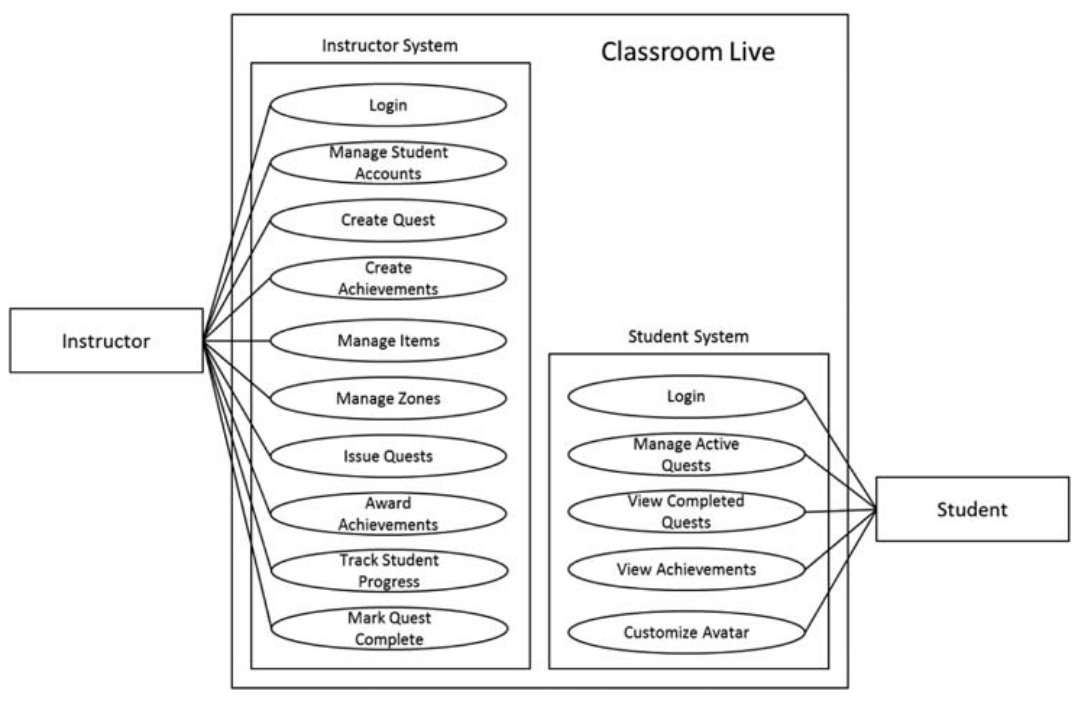
\includegraphics[width=1\textwidth]{imagens/classroom_diagrama.png}
\source{\citet{de2013classroom}}
\label{fig:classroom_diagrama}
\end{figure}

A Figura \ref{fig:classroom_diagrama} demonstra as funcionalidades existentes no sistema para o aluno e o instrutor. Após o instrutor acessar o sistema, ele utiliza cinco áreas do sistema para planejar uma nova aula. Na área \textit{”Manage Student Accounts”}, o instrutor pode criar novas contas de usuário e configurar contas já existentes. A área \textit{“Create Quest”} é onde o instrutor passará a maior parte do tempo, pois é nesta área onde é realizada a criação de novas \textit{quest} a serem completadas pelo alunos. Neste processo, o instrutor tem a possibilidade de relacionar recompensas e pontos de experiência que o aluno receberá ao completar a \textit{quest}. 

A área \textit{“Create Achievements”}, permite ao instrutor criar uma biblioteca de recompensas e associar pontos de experiência a elas. As áreas \textit{“Manage Itens”} e \textit{“Manage zones”} permitem ao instrutor manipular os itens virtuais e os ambientes visuais que o aluno encontrará durante utilização do sistema.

Durante as aulas, o instrutor terá quatro áreas para gerenciar as atividades dos alunos. Na área \textit{“Issue Quest”}, o instrutor poderá controlar as \textit{quests} existentes, podendo inativa-las, definir um tempo limite para a conclusão. Na área \textit{”Award Achievements”}, o instrutor tem a possibilidade de definir prêmios para os alunos. Na área \textit{“Track Student Progress”}, o instrutor pode observar o avanço dos alunos. Na última área, \textit{"Mark quest"} complete, o instrutor analisa o trabalho realizado pelo estudante e define se este cumprir com a especificação determinada ou não.

Na sessão do alunos, existem 4 funcionalidades. A principal delas é a \textit{“Manege Active Quests”}, esta é a funcionalidade que permite o alunos visualizar suas \textit{quests} e enviar suas respectivas respostas. A funcionalidade \textit{“View Completed Quests”} possibilita ao aluno visualizar sua própria performance em \textit{quests} já concluídas, e também permite a visualização das respostas corretas paras as \textit{quests}. A funcionalidade \textit{“View Achievements”} permite a visualização de todas as conquista recebidas pelo usuário. Por final, a funcionalidade “Customize Avatar” é onde o aluno pode customizar a aparência de seu avatar a partir dos itens conquistados.

Para avaliar a eficácia do Classroom Live, os autores aplicaram a ferramenta em uma parte do curso de introdução a programação. A Figura \ref{fig:classroom_aula}, demonstra a sequência de eventos utilizados nesta experiência de aplicação em sala de aula. Cada lição começa com a criação de dois tipos de \textit{quests} por parte do instrutor. O primeiro corresponde a uma tarefa onde o aluno deve desenvolver e enviar um trecho de código fonte que corresponda a tarefa atribuída. O instrutor também desenvolve \textit{quests} de múltiplas escolhas relacionadas ao material ensinado na aula daquele dia. O instrutor tem a possibilidade de adicionar recompensas em ambas as \textit{quests}.

Quando o aluno submete suas respostas, os resultados são enviados automaticamente para o servidor para que instrutor possa realizar a revisão do que foi feito. Dependendo da performance dos estudantes, o instrutor por decidir se deve ou não voltar para a explicação teórica ou mover para o próximo tópico. Enquanto isso, os alunos recebem \textit{feedback} de suas ações realizadas. A atribuição de recompensas é realizada pelo instrutor após ele realizar a revisão da tarefa completada pelo aluno.

\begin{figure}[ht]
\centering
\caption{\textbf{Sequência de eventos aplicados em sala de aula}}
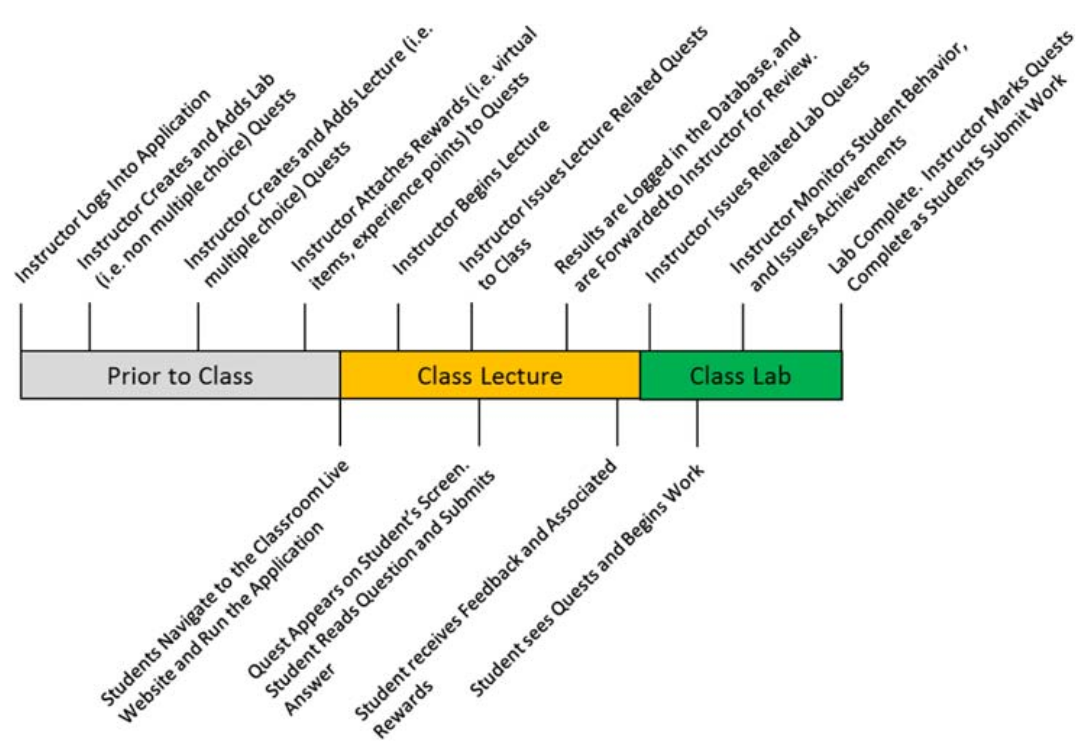
\includegraphics[width=0.9\textwidth]{imagens/classroom_aula.png}
\source{\citet{de2013classroom}}
\label{fig:classroom_aula}
\end{figure}

Durante a aplicação do sistema Classroom Live no curso de introdução a programação, durante 5 meses, os autores identificaram diversas lições aprendidas de quão eficiente pode ser a utilização de gamificação na sala de aula. Dentre elas estão:

O conteúdo é muito importante: A eficácia da aplicação da ferramenta depende da habilidade de gerar conteúdo atraente para os alunos. Os estudantes demonstram um maior interesse quando as \textit{quest} eram instigantes e recompensados. Os autores encontraram uma relação entre o engajamento dos alunos e o conteúdo, como grande volumes de \textit{quests} e recompensas os alunos demonstravam maior participação.

Gamificação demanda tempo: Segundo os autores, as utilização de gamificação na sala de aula aumentou o tempo necessário para a preparação das aulas, mesmo com a utilização de um software como Classroom Live para auxiliar. Para estas aulas, os instrutores tiveram que popular o sistema com itens e \textit{quests} que deveriam ser atraentes para os alunos e relevantes para o curso. Os autores acreditam que este tempo diminuirá à medida que é construída uma base de dados de \textit{quests} que possam ser reutilizadas em outros semestres.

Para avaliar a aplicação, foi solicito para que os alunos responder algumas questões referente a utilização do Classroom Live, como pode ser visualizado na Figura \ref{fig:classroom_avaliacao}. O estudo realizado com 15 alunos.

\begin{figure}[ht]
\centering
\caption{\textbf{Avaliação da ferramenta}}
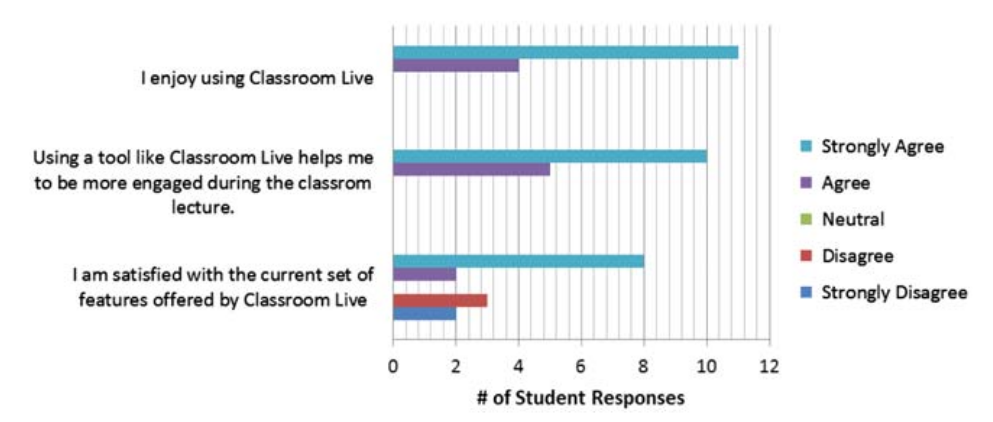
\includegraphics[width=0.9\textwidth]{imagens/classroom_avaliacao.png}
\source{\citet{de2013classroom}}
\label{fig:classroom_avaliacao}
\end{figure}

Segundo os autores, aparentemente os alunos gostaram de utilizar o Classroom Live. As respostas das duas primeiras questões indicam que os alunos acharam o Classroom Live divertido e acreditam que o software auxiliou a mantê-los engajados na aula. Levando em consideração que o uso do software foi totalmente voluntário, os autores constataram o entorno de 85\% dos alunos utilizaram a aplicação e participaram de \textit{quests} durante todas as aulas. 

Os autores não conseguiram constatar se a utilização da ferramenta aumentou a performance dos estudantes, mas eles observaram que a aplicação obteve êxito em relação a melhorar o interesse e engajamento dos estudantes nas aula.

\section{Considerações}
Neste capítulo foi apresentado ferramentas relacionadas ao trabalho desenvolvido, cumprindo, desta forma, o terceiro objetivo específico do trabalho. Foi abordado o funcionamento das ferramente e como elas foram utilizadas em sala de aula.

No próximo capítulo será apresentado a proposta do trabalho. Será demonstrando o principal objetivo do trabalho e o que será feito para cumpri-lo, abordando quais elementos da gamificação serão utilizados e como serão implementados na ferramenta.

% ----------------------------------------------------------
% Proposta
% ----------------------------------------------------------
\chapter{Proposta} 

O objetivo principal deste trabalho é o desenvolvimento de uma ferramenta gamificada para o auxílio ao ensino de processamento digital de imagens. Primeiramente foi realizado um estudo de sistemas com objetivos semelhantes e os principais conceitos de gamificação que serviram como aporte para o desenvolvimento da proposta. Estes estudos foram apresentados nos capítulos anteriores.
    
Este trabalho fará uso da ferramenta VISNode (apresentada na sessão \ref{sec:visnode}). Esta ferramenta já se encarra de proporcionar um ambiente para a prototipação e experimentação de técnicas de PDI, possuindo diversas técnicas já implementadas. 
   
% ---
\section{VISNode}
\label{sec:visnode}

Esta ferramenta foi desenvolvida por alunos da Universidade Feevale após concluírem a disciplina de Processamento Digital de Imagem. Eles identificaram uma dificuldade para realizar a comparação de técnicas, com o mesmo objetivo, e escolher o parâmetro adequada para cada situação. Desta forma, foi desenvolvido um ferramenta que tem por objetivo demonstrar, de forma visual,  a execução de técnicas de PDI e como elas se conectam \cite{visnode}.

O VISNode utiliza o conceito de processos, que consiste em operações que podem ser executados em entradas (\textit{inputs}) e gerar saídas (\textit{outputs}). Estas saídas podem ser imagens, valores numéricos, ou qualquer outra estrutura de dados necessária para a execução do processo. Os processos podem ser qualquer função que possa ser aplicada a um \textit{input} e gerar um \textit{output}, como por exemplo: de manipulação da imagem, como desfoque de Gauss, limiarização ou de inversão de cores; obtenção de informações, como a obtenção de estatísticas de cor;  extração de objetos \cite{visnode}.

Cada processo da ferramenta é considerado um nodo, como em uma árvore ou grafo. Cada nodo possui entradas e saídas que podem ser conectadas a entradas e saídas de outros nodos para a execução sequencial. Para um processo de Threshold, por exemplo, a imagem de origem e o limiar numérico são os parâmetros de entrada, enquanto a imagem resultante da operação consiste no parâmetro de saída \cite{visnode}. 

Para determinados tipos de entrada é possível informar o valor manualmente no nodo ou via conexão. Por exemplo, para o nodo de limiarização é possível informar um valor numérico para o limiar diretamente no nodo, utilizando a interface gráfica, ou obter à partir da saída de outro nodo, como, por exemplo, a cor média da imagem \cite{visnode}.

Segundo os criadores, a estrutura em nodos foi criada com o intuito de facilitar a compreensão em relação a como diversos processos podem ser executados de forma sequencial para chegar a um objetivo final. Na tela principal de edição do software, o usuário pode mover, inserir e remover nodos de processos, criar e remover conexões entre as entradas e saídas de forma visual e realizar ajustes nos parâmetros dos processos, visualizando em tempo real o resultado de suas modificações.

A Figura \ref{fig:visnode} demonstra a utilização do software VISNode. Nesta figura é possível visualizar um painel, à direita do software, de onde é possível selecionar as técnicas de PDI a serem aplicadas na imagem. Também é demonstrado um fluxo de execução utilizando duas técnicas: \textit{Grayscale} e \textit{Threshold}. No processo de \textit{Threshold} é possível observar um \textit{input slider} por onde é realizado a mudança do parâmetro do limiar.

\begin{figure}[ht]
\centering
\caption{\textbf{Demonstrativo do VISNode}}
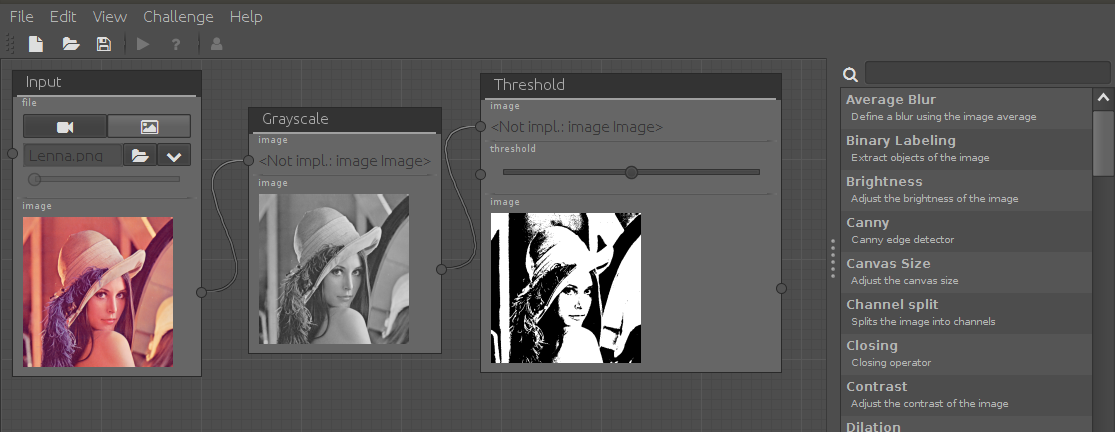
\includegraphics[width=0.9\textwidth]{imagens/visnode.png}
\sourceAuthor
\label{fig:visnode}
\end{figure}

% ---
\subsection{Arquitetura}

O software VISNode foi construído utilizando a arquitetura modular proposta por Reis et al. (2017), onde é construída uma linha de produtos de software (\textbf{Software Product Line} ou SPL) (SEI, 2018)  para a extração e apresentação de características em exames médicos por imagem. Na arquitetura existem cinco módulos, cada um com um objetivo específico, que podem ser usados de forma independente para diversos tipos de aplicações que trabalham com imagens. Dos módulos construídos, três foram utilizados no desenvolvimento do VISNode, descritos a seguir:

PDI: implementações de algoritmos de processamento de imagens, que são aplicados aos exames médicos no processo de extração de características, como, por exemplo: histograma, limiarização, remoção e redução de ruídos, operações de convolução, métodos de classificação, entre outros \cite{reisferramenta}; 

\begin{enumerate}
\item Uso Comum: classes de uso  comum  por todos os outros módulos, como classes utilitárias ou estruturas de dados utilizadas na troca de informações entre módulos; 
\item Acesso a Arquivos: camada de acesso arquivos do tipo DICOM.
\end{enumerate}

% ---
\section{Proposta gamificada}

O presente trabalho se propõe a desenvolver uma ferramenta que faça uso de conceitos de gamificação visando auxiliar o ensino e aprendizagem. Este trabalho foca no ensino de processamento digital de imagens, pretendendo servir como aporte para alunos de disciplinas que abordam esses conceitos.

Tendo como objetivo dar assistência ao usuário no entendimento dos algoritmos utilizados, a ferramenta provê informações detalhadas dos algoritmos implementados, sendo possível visualizar uma explicação textual de seu funcionamento, além do código de sua implementação. Esta funcionalidade também pode servir como material didático, auxiliando na etapa de aprendizado de usuários como pouca conhecimento na área.

\subsection{Elementos}

O principal objetivo do trabalho é desenvolver um ferramenta que motive os alunos a participarem das aulas e engaja-los na busca por conhecimentos relacionados a área de estudo. Para isso será utilizada a gamificação. A ferramenta contará com elementos como: Desafios, Missões, Narrativas, Recompensas e Rankings.

\subsubsection{Desafios}

A ferramenta irá contar com desafios. Um desafio consiste em uma tarefa que o usuário deverá realizar. Cada desafio possuirá uma narrativa, na qual deve contextualizar o problema visando motivar o usuário à resolução do mesmo.

A resolução do desafio deve ser realizada utilizando o VISNode, desta forma, o usuário deverá conectar as técnicas existente para obter o resultado esperado. O próprio software realizará a conferência se a solução proposta pelo usuário condiz com o resultado esperado. Informações como número de tentativa e duração serão armazenadas para análises por parte do educador.

\subsubsection{Missões}

Um missão consiste em um grande objetivo que o usuário deve alcançar. Cada missão será composta por desafios, desta forma, para um usuário concluir uma missão, este deverá concluir primeiramente uma seŕie de pequenos desafios. Estes desafios são pensados para que o aluno consiga dividir o problema em partes, desta forma, a resolução de um problema de maior complexidade é mais facilmente alcançada.

Cada missão possuirá uma narrativa para que seja apresentado ao aluno a problemática a ser trabalhada. Esta narrativa irá descrever o problema como um todo e irá demonstrar o resultado final esperado. Abaixo será apresentado um exemplo de missão.

\subsubsection{Narrativa} 
Uma loja procura uma maneira mais simples de calcular o valor em moedas existes em suas caixas registradoras. A cada encerramento de caixa, fica a cargo do operador realizar a conferência que quanto em valor existe em cada caixa. Levando em consideração este cenário, foi desenvolvido um equipamento que possui um câmera fotográfica a cima de um tablado. Pede-se para desenvolver um algoritmo de processamento digital de imagens que seja capaz de identificar cada moeda e calcular o valor existente no tablado. A Figura \ref{fig:exemploNarrativa} apresenta um exemplo da imagem capturada do tablado. 

\begin{figure}[ht]
\centering
\caption{\textbf{Imagem capturada do equipamento de cálculo de valor monetário}}
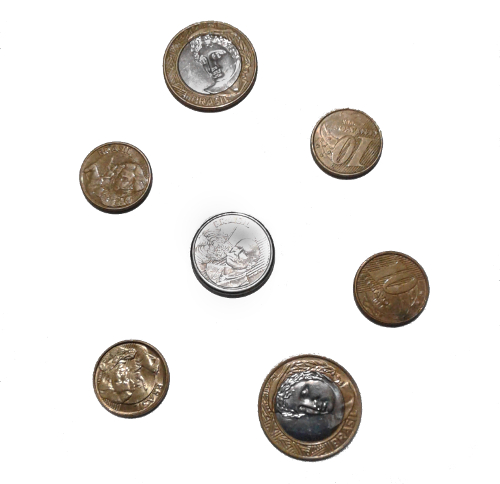
\includegraphics[width=0.8\textwidth]{imagens/moedas.jpg}
\sourceAuthor
\label{fig:exemploNarrativa}
\end{figure}


\subsubsection{Desafios}

\begin{enumerate}
\item \textbf{Pré-processamento}: Neste desafio os usuários terão de trabalhar para melhorar a qualidade da imagens para que seja possível realizar o processo de segmentação. Como resultado espera-se que seja retornado uma imagem binária, onde os pixels com valor 0 correspondam ao fundo da imagem, e os pixels com valor 1 correspondam as moedas.
\item \textbf{Cálculo do valor}: Neste desafios os usuários terão que executar algum procedimento que realize a segmentação das imagens. Após este procedimento, deveram extrair características de cada objeto para que seja possível identificar qual é o valor monetário de cada imagem.
\end{enumerate}

\subsubsection{Recompensas e pontos de experiência}

Ao completar missões e desafios o usuário receberá pontos de experiência. Cada tarefa terá sua pontuação de acordo com o grau de dificuldade imposto ao usuário. Esta informação de experiência transmite ao usuário um \textit{feedback} de como ele está em relação ao seu progresso. Além de ser um fator de motivação extrínseca. 

Além dos pontos de experiência, o usuário poderá receber algumas recompensas. Um exemplo de recompensa seria o usuário receber um parte de uma imagem a cada desafio completado. Após a conclusão de alguns desafios, o usuário possuirá a imagem completa.

\subsubsection{Rankings}

Tendo em visa a possibilidade do usuário se situar em relação ao seu desempenho comparado com outros usuários, a ferramenta possuirá um ranking. Este ranking levará em consideração a pontuação conquistada por cada usuário para posiciona-los em suas respectivas colocações.


\subsection{Utilização}

A parte gamificada da ferramenta será acessar através de um cadastro e login no sistema. Isso se torna necessário para poder identificar o usuário que esta acessando o sistema, e também para controlar o progresso de cada usuário. Após o usuário logado, ele terá acesso a todas as funcionalidades referentes a parte gamificada da ferramenta.

Logado no sistema, o usuário possui acesso ao menu de missões. Neste local o usuário encontrará diversas missões com diferentes objetivos e graus de dificuldades diferentes. O usuário poderá selecionar uma missão para ser realiza e cada conquista receberá suas respectivas recompensas.

A ferramenta exibirá os pontos do usuário na página principal do sistema. Isso ocorrerá para que os usuário recebem um \textit{feedback} o mais rápido possível.

O usuário terá acesso a dois menus responsável pelo ranking e uma lista das recompensas conquistas pelo usuário. Também haverá uma página onde o usuário poderá visualizar seu progresso em cada missão, sendo possível visualizar o quanto ele já cumpriu de cada missão.

Quando a ferramenta for utilizada dentro da sala de aula, o educador poderá criar um grupo de trabalho e definir quais usuário e quais desafios este grupo irá compor. Desta forma, o educador poderá controlar o progresso de cada participante do grupo, podendo visualizar quantas tarefas o usuário já realizou, como ele solucionou os desafios e quais recompensas ele já ganhou.

Visando ser utilizada em outras instituições, a ferramenta permite a criação de novas missões e desafios. Ampliando, desta forma, o uso da ferramenta para mais usuários.

A ideia da ferramenta é que possa ser utilizada dentro da sala de aula, como já descrito, mas também fora. Para isso, a ferramenta contará com áreas que podem ser acessíveis por pessoas fora da disciplina. Desta forma, qualquer indivíduo que tenha interesse em utilizar a ferramenta poderá utiliza-la.

\subsection{Validação}

A validação da ferramenta será realizada dentro de sala de aula. Para isso, será elaborado uma aula onde os alunos da disciplina irão utilizar a ferramenta como meio de aprendizagem. Serão propostas missão ao alunos.

Esta validação busca identificar se a utilização da ferramenta pode auxiliar os alunos no ensino e aprendizagem de PDI. Verificar se sua utilização auxiliou na motivação dos estudante em relação a conteúdo da disciplina.

Após a utilização do ferramenta, será aplicado ao estudantes um questionário sobre a utilização da ferramenta. Este questionário será focado em avaliar se, na percepção dos estudantes, a ferramenta foi útil ou não.

Também será solicitado ao educador avaliar a experiência da aplicação da ferramenta em sala de aula. Esta avaliação tem por objetivo extrair a percepção do avaliador em relação ao uso da ferramenta.

\section{Considerações}

Neste capítulo foi apresentado a proporta do trabalho, cumprindo, desta forma, o quarto objetivo específico do trabalho. Foi demonstrando o principal objetivo do trabalho e o que será feito para cumpri-lo, abordando quais elementos da gamificação serão utilizados e como serão implementados na ferramenta.

No próximo capitulo será apresentado o desenvolvimento da ferramenta. Será demonstrado o as tecnologias envolvidas no desenvolvimento e as etapas realizadas até a conclusão do desenvolvimento e o resultado final da implementação.

% ----------------------------------------------------------
% Desenvolvimento
% ----------------------------------------------------------
\chapter{Desenvolvimento} 

%https://invis.io/XWGWAN156ES#/291345781_01

% ---
\section{Arquitetura}
Acesso a dados

\begin{figure}[ht]
\centering
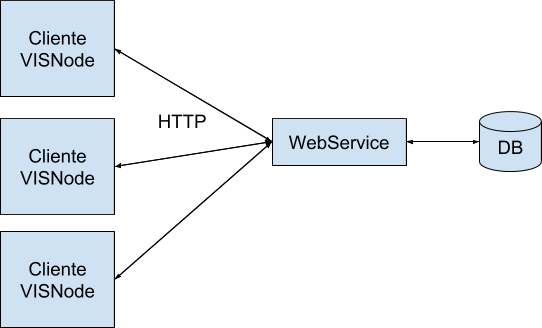
\includegraphics[width=1\textwidth]{imagens/visnode_arquitetura.png}
\end{figure}

% ---
\section{\textit{Ranking}}

\textit{ranking} geral
Top 10: Os 10 mais bem colocados 
Posição do usuário
\textit{ranking} por grupo
Lista de todos os participantes, posicionando a página na posição do usuário (acredito que não vai ter muitos usuários neste cenário) 

\begin{figure}[ht]
\centering
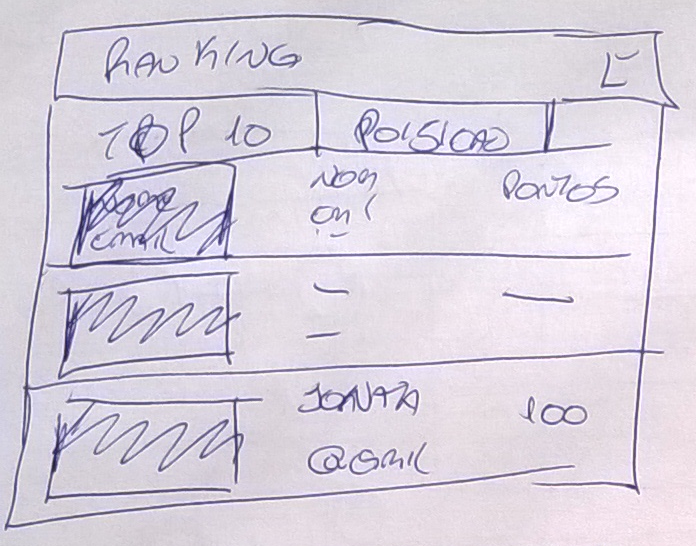
\includegraphics[width=1\textwidth]{imagens/proposta_ranking.png}
\end{figure}

% ---
\section{Progresso}

Usuário precisa ter uma noção de seus progresso
Exibir um formato de lista o percentual realizado das missões 

\begin{figure}[ht]
\centering
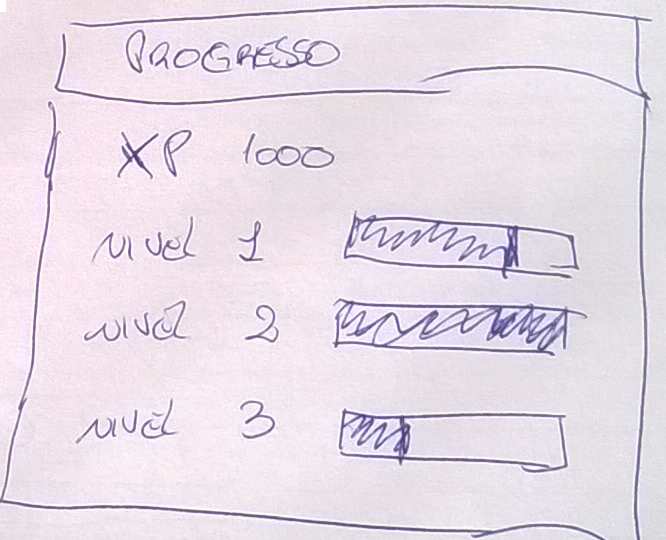
\includegraphics[width=1\textwidth]{imagens/proposta_progresso.png}
\end{figure}

% ---
\section{Recompensas}

Imagem definida para a missão
A imagem será quebrada em formato de quebra cabeça e dada ao usuário a medida que ele vai completando as missões
Definir a quantidade de peças
Pontos
Ao completar desafios
Ao completar missões

\begin{figure}[ht]
\centering
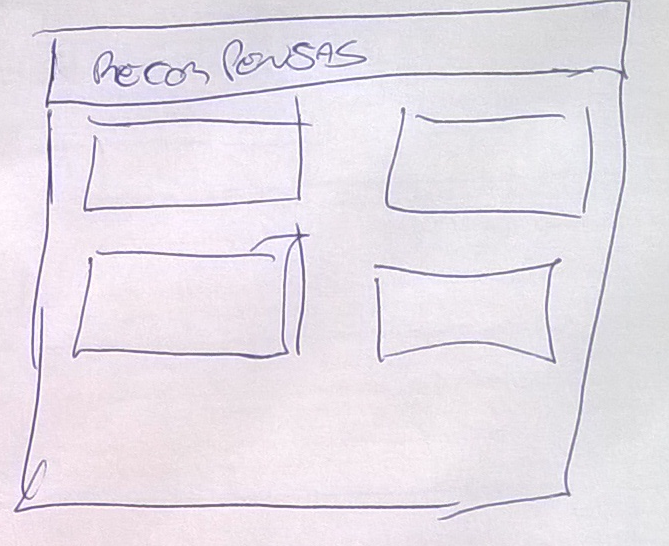
\includegraphics[width=1\textwidth]{imagens/proposta_recompensa.png}
\end{figure}

\begin{figure}[ht]
\centering
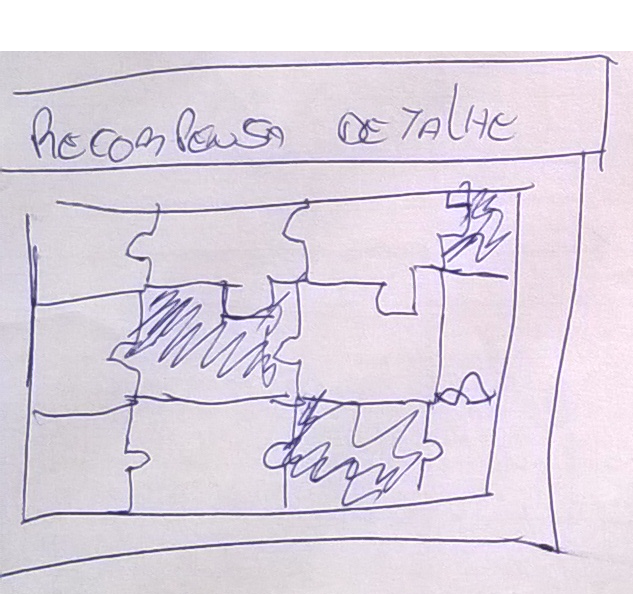
\includegraphics[width=1\textwidth]{imagens/proposta_recompensa_detalhe.png}
\end{figure}

% ---
\section{Cadastro}


Alguns usuários poderão criar grupos de trabalhos
Definir quais usuário
Definir quais missões
Definir recompensas das missões
Criar nova missões

\begin{figure}[ht]
\centering
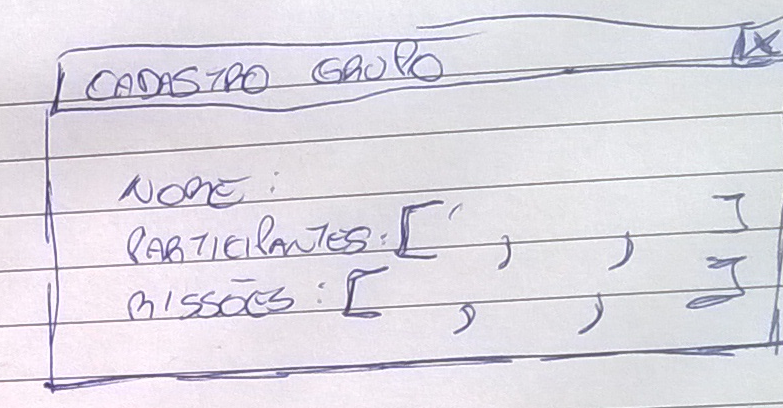
\includegraphics[width=1\textwidth]{imagens/proposta_cadastro.png}
\end{figure}

\begin{figure}[ht]
\centering
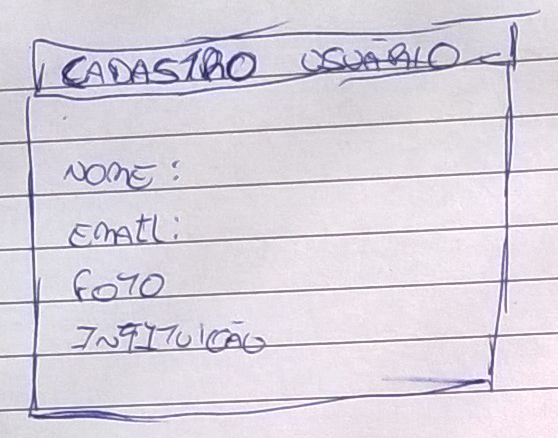
\includegraphics[width=1\textwidth]{imagens/proposta_cadastro_usuario.png}
\end{figure}

% ---
\section{Missões}

Poder conter N objetivos
Narrativa
Desafios
Questionario
Desenvolvimento VISNode
Narrativa inicial
Texto
Imagem
Nível de dificuldade (Básico, Intermediário, Avançado)
Visibilidate
Global
Grupo de trabalho

\begin{figure}[ht]
\centering
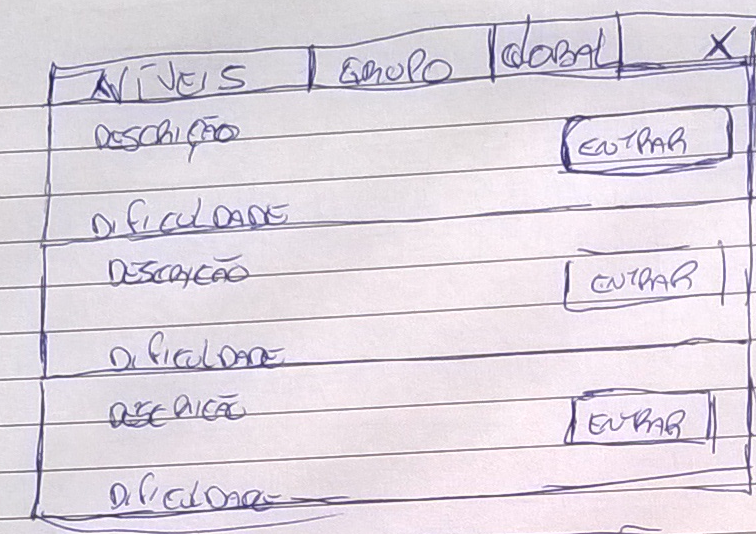
\includegraphics[width=1\textwidth]{imagens/proposta_niveis.png}
\end{figure}

\begin{figure}[ht]
\centering
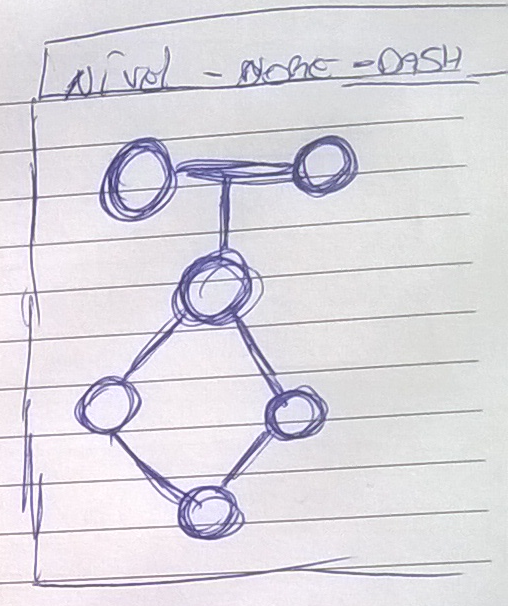
\includegraphics[width=1\textwidth]{imagens/proposta_nivel.png}
\end{figure}

\begin{figure}[ht]
\centering
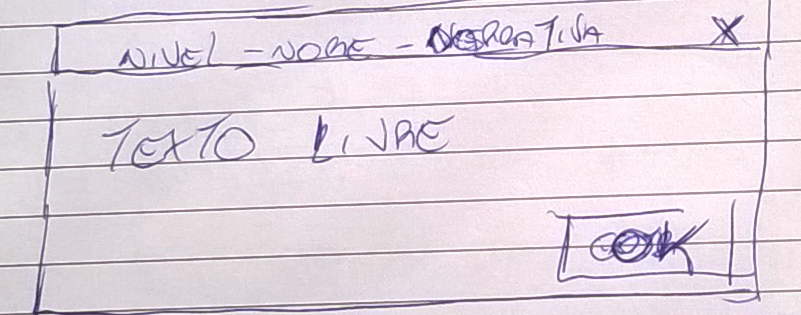
\includegraphics[width=1\textwidth]{imagens/proposta_narrativa.png}
\end{figure}

\begin{figure}[ht]
\centering
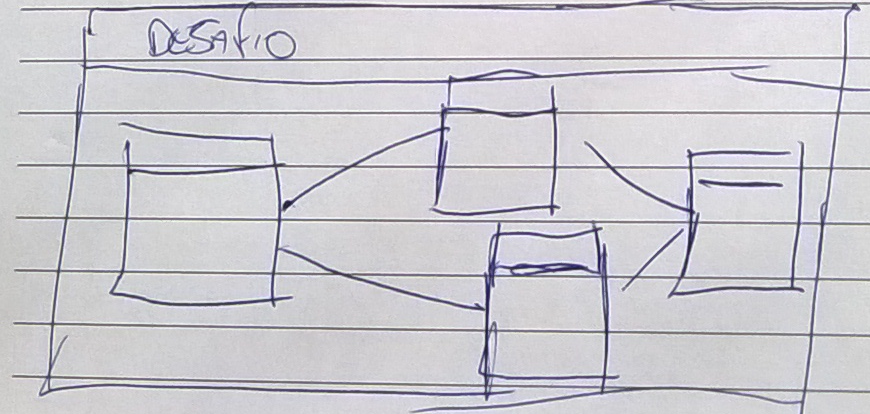
\includegraphics[width=1\textwidth]{imagens/proposta_desafio.png}
\end{figure}

\begin{figure}[ht]
\centering
\includegraphics[width=1\textwidth]{imagens/proposta_desafio_questionario.png}
\end{figure}

\begin{figure}[ht]
\centering
\includegraphics[width=1\textwidth]{imagens/proposta_tarefa_descricao.png}
\end{figure}

% ---
% Finaliza a parte no bookmark do PDF, para que se inicie o bookmark na raiz
% ---
\bookmarksetup{startatroot}% 
% ---

% ---
% Conclusão
% ---
\chapter*[Conclusão]{Conclusão}
\addcontentsline{toc}{chapter}{Conclusão}

\lipsum[31-33]

% ----------------------------------------------------------
% ELEMENTOS PÓS-TEXTUAIS
% ----------------------------------------------------------
\postextual


% ----------------------------------------------------------
% Referências bibliográficas
% ----------------------------------------------------------
\bibliography{abntex2-modelo-references}


%---------------------------------------------------------------------
% INDICE REMISSIVO
%---------------------------------------------------------------------

\printindex

\end{document}
